\thispagestyle{thachthuctoanhocnone}
\pagestyle{thachthuctoanhoc}
\everymath{\color{thachthuctoanhoc}}
\graphicspath{{../thachthuctoanhoc/pic/}}
\begingroup
\AddToShipoutPicture*{\put(0,616){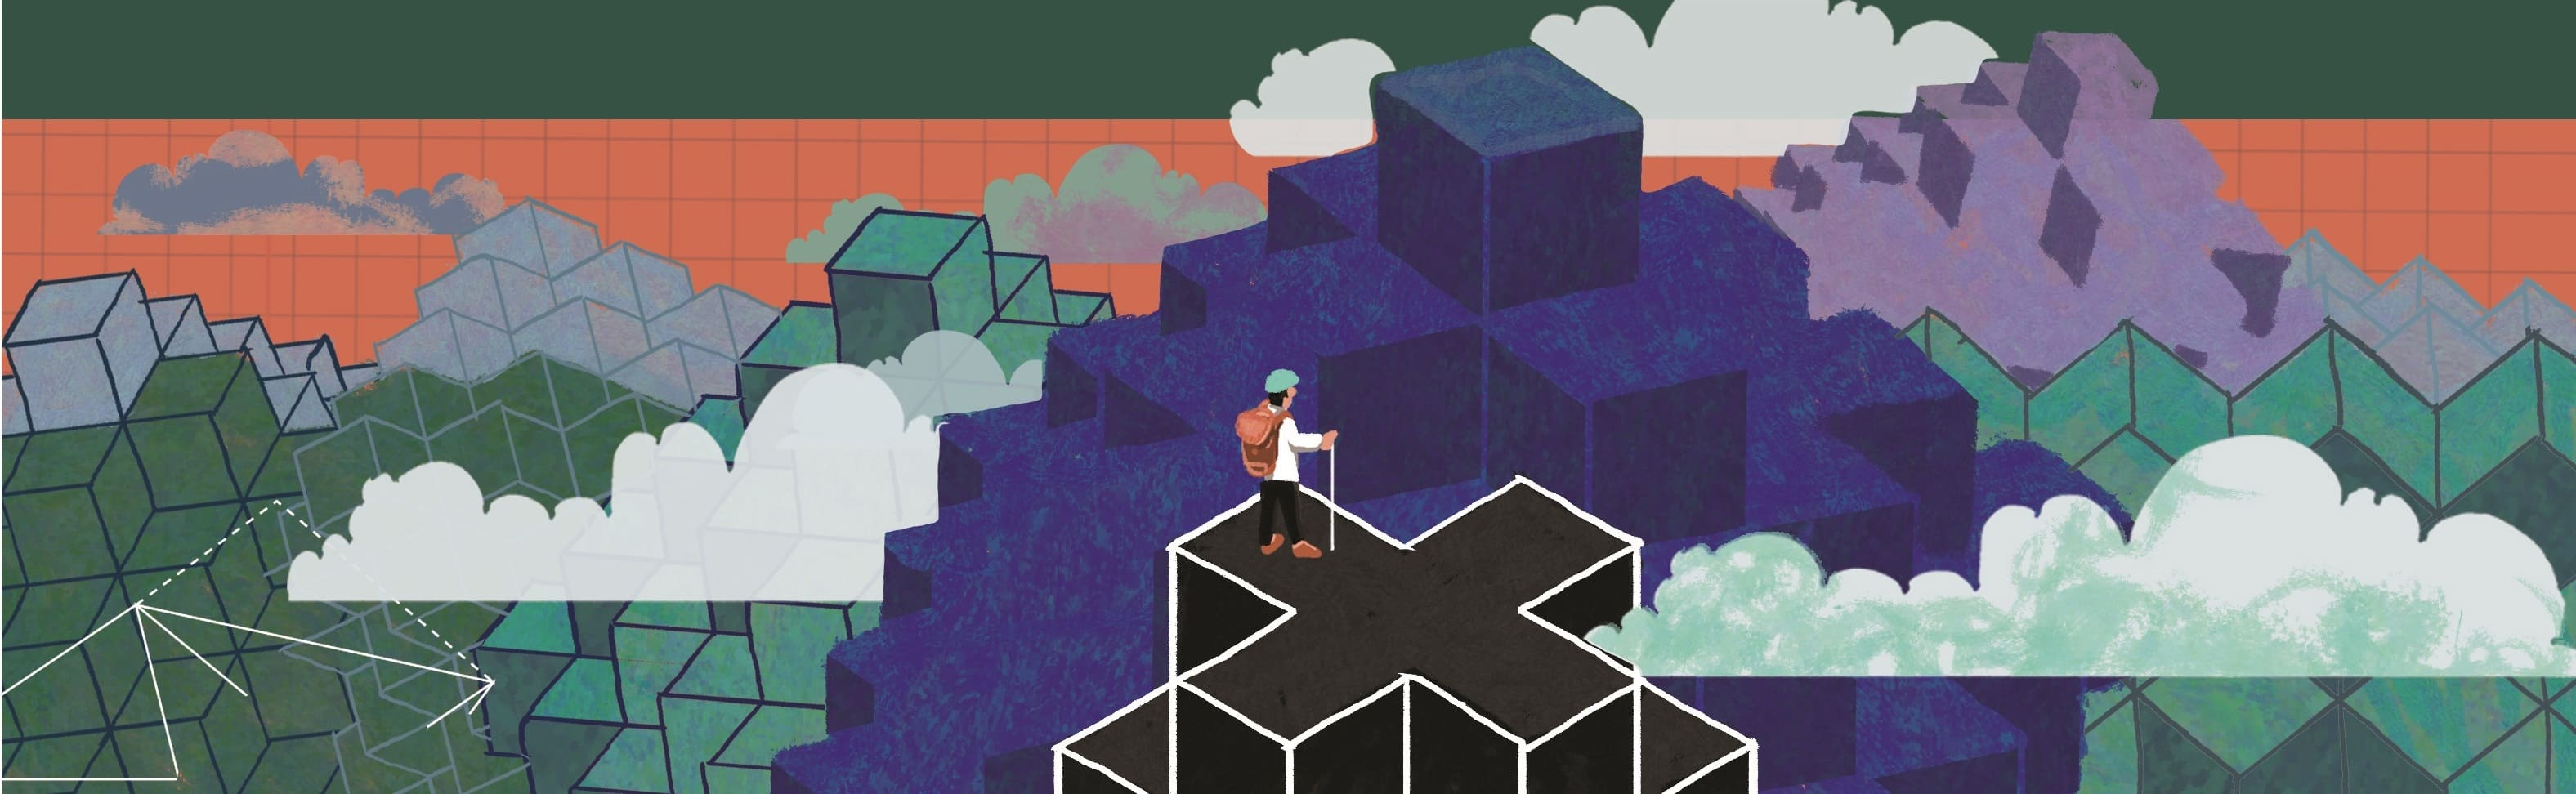
\includegraphics[width=19.3cm]{../thachthuctoanhoc/bannerthachthuc}}}
\centering
\vspace*{4cm}
\endgroup
\vspace*{-8pt}
\begin{tBox}
	\begin{itemize}[leftmargin = 13pt, itemsep = 1.0pt] 
				\item Mỗi bài toán đề xuất (kèm theo lời giải) cần được nêu rõ là bài sáng tác hay bài sưu tầm.
%		\item Mỗi bài toán đề xuất (kèm theo lời giải) cần được nêu rõ là bài sáng tác hay bài sưu tầm (nếu là bài sưu tầm, cần ghi rõ nguồn).
		\item Bài giải cho mỗi bài toán cần được trình bày trong một file riêng hoặc
		một tờ giấy riêng.
		\item  Người đề xuất bài toán hoặc gửi bài giải cho các bài toán trong mục ``Thách thức kỳ này" cần ghi rõ họ, đệm, tên và nơi làm việc/học tập, số điện thoại liên hệ. Nếu là học sinh (hoặc sinh viên) cần ghi rõ là học sinh lớp mấy (hoặc sinh viên năm thứ mấy).
		\item Các bài toán trong mục Thách thức kỳ này hướng tới các độc giả là học sinh phổ thông; được phân chia thành các mức độ $B$, $A$, và được sắp xếp theo độ khó tăng dần, theo đánh giá chủ quan của Ban biên tập. Các bài toán mức độ $B$ không đòi hỏi các kiến thức vượt quá chương trình môn Toán cấp THCS; các bài toán mức độ $A$ không đòi hỏi các kiến thức vượt quá chương trình môn Toán cấp THPT.
		\item Cách thức gửi bài toán đề xuất hoặc lời giải: gửi file thu được bằng cách scan, ảnh chụp (rõ nét) của bản viết tay, hoặc được soạn thảo bằng các phần mềm Latex, Word tới \url{bbt@pi.edu.vn} hoặc gửi qua đường bưu điện tới Tòa soạn (xem địa chỉ tại bìa $2$).
		\item Hạn gửi lời giải cho các bài toán P$631$--P$640$: trước ngày $15/10/2022$.
	\end{itemize}
\end{tBox}
\begin{center}
	\vspace*{-5pt}
	\textbf{\color{thachthuctoanhoc}\color{thachthuctoanhoc}THÁCH THỨC KỲ NÀY}
	\vspace*{-5pt}
\end{center}
\begin{multicols}{2}
	\setlength{\abovedisplayskip}{4pt}
	\setlength{\belowdisplayskip}{4pt}
	{\color{thachthuctoanhoc}{\usefont{T5}{qag}{b}{n} P631.}}
	(Mức $B$) Các số tự nhiên, bắt đầu từ $20$, được viết liên tiếp nhau thành một hàng ngang, như sau:
	\begin{align*}
		2021222324252627\ldots.
	\end{align*}
	Hỏi chữ số ở vị trí thứ $2022$, kể từ trái qua phải, là chữ số nào?
	\begin{flushright}
		\textit{Hoàng Ngự Huấn, Hà Nội (st)}
	\end{flushright}
	{\color{thachthuctoanhoc}{\usefont{T5}{qag}{b}{n} P632.}}
	(Mức $B$) Cho $x,y,z$ là các số thực dương thoả mãn 
	\begin{align*}
		\dfrac{x^2}{(x+y)^2}+\dfrac{y^2}{(y+z)^2}+\dfrac z{z+x}=1.
	\end{align*}
	Chứng minh rằng $x=y=z$. 
	\begin{flushright}
		\textit{Trần Quốc Luật, Tp. Hồ Chí Minh}
	\end{flushright}
	{\color{thachthuctoanhoc}{\usefont{T5}{qag}{b}{n} P633.}}
	(Mức $B$) Chứng minh rằng, với mọi số nguyên dương $n$, số dư trong phép chia số $A=n^{2024}+n^{2025}$  cho số $B=n+n^2+n^3+\cdots+n^{2022}$ là một số chẵn. 
	\vskip 0.05cm
	\hfill	\textit{Cao Ngọc Toản, Thừa Thiên Huế}
	\vskip 0.05cm
	{\color{thachthuctoanhoc}{\usefont{T5}{qag}{b}{n} P634.}}
	(Mức $B$) Bạn Pi muốn ghi số $4$ vào hình tròn nhỏ, nằm ở tâm của đường tròn lớn trong Hình dưới đây. Sau đó, Pi muốn ghi tiếp vào mỗi hình tròn nhỏ còn lại một số nguyên, sao cho hai điều kiện sau được đồng thời thoả mãn: 
	\vskip 0.05cm
	$i.$ Tổng của tám số ở tám hình tròn nhỏ nằm trên đường tròn lớn bằng $66$. 
	\vskip 0.05cm
	$ii.$ Tổng của ba số ở ba hình tròn nhỏ, nằm trên cùng một đường kính của đường tròn lớn, đều bằng nhau. 
	\vskip 0.05cm
	Hỏi, Pi có thể thực hiện được ý muốn của mình hay không? Vì sao?
	\begin{figure}[H]
		\centering
		\vspace*{-5pt}
		\captionsetup{labelformat= empty, justification=centering}
		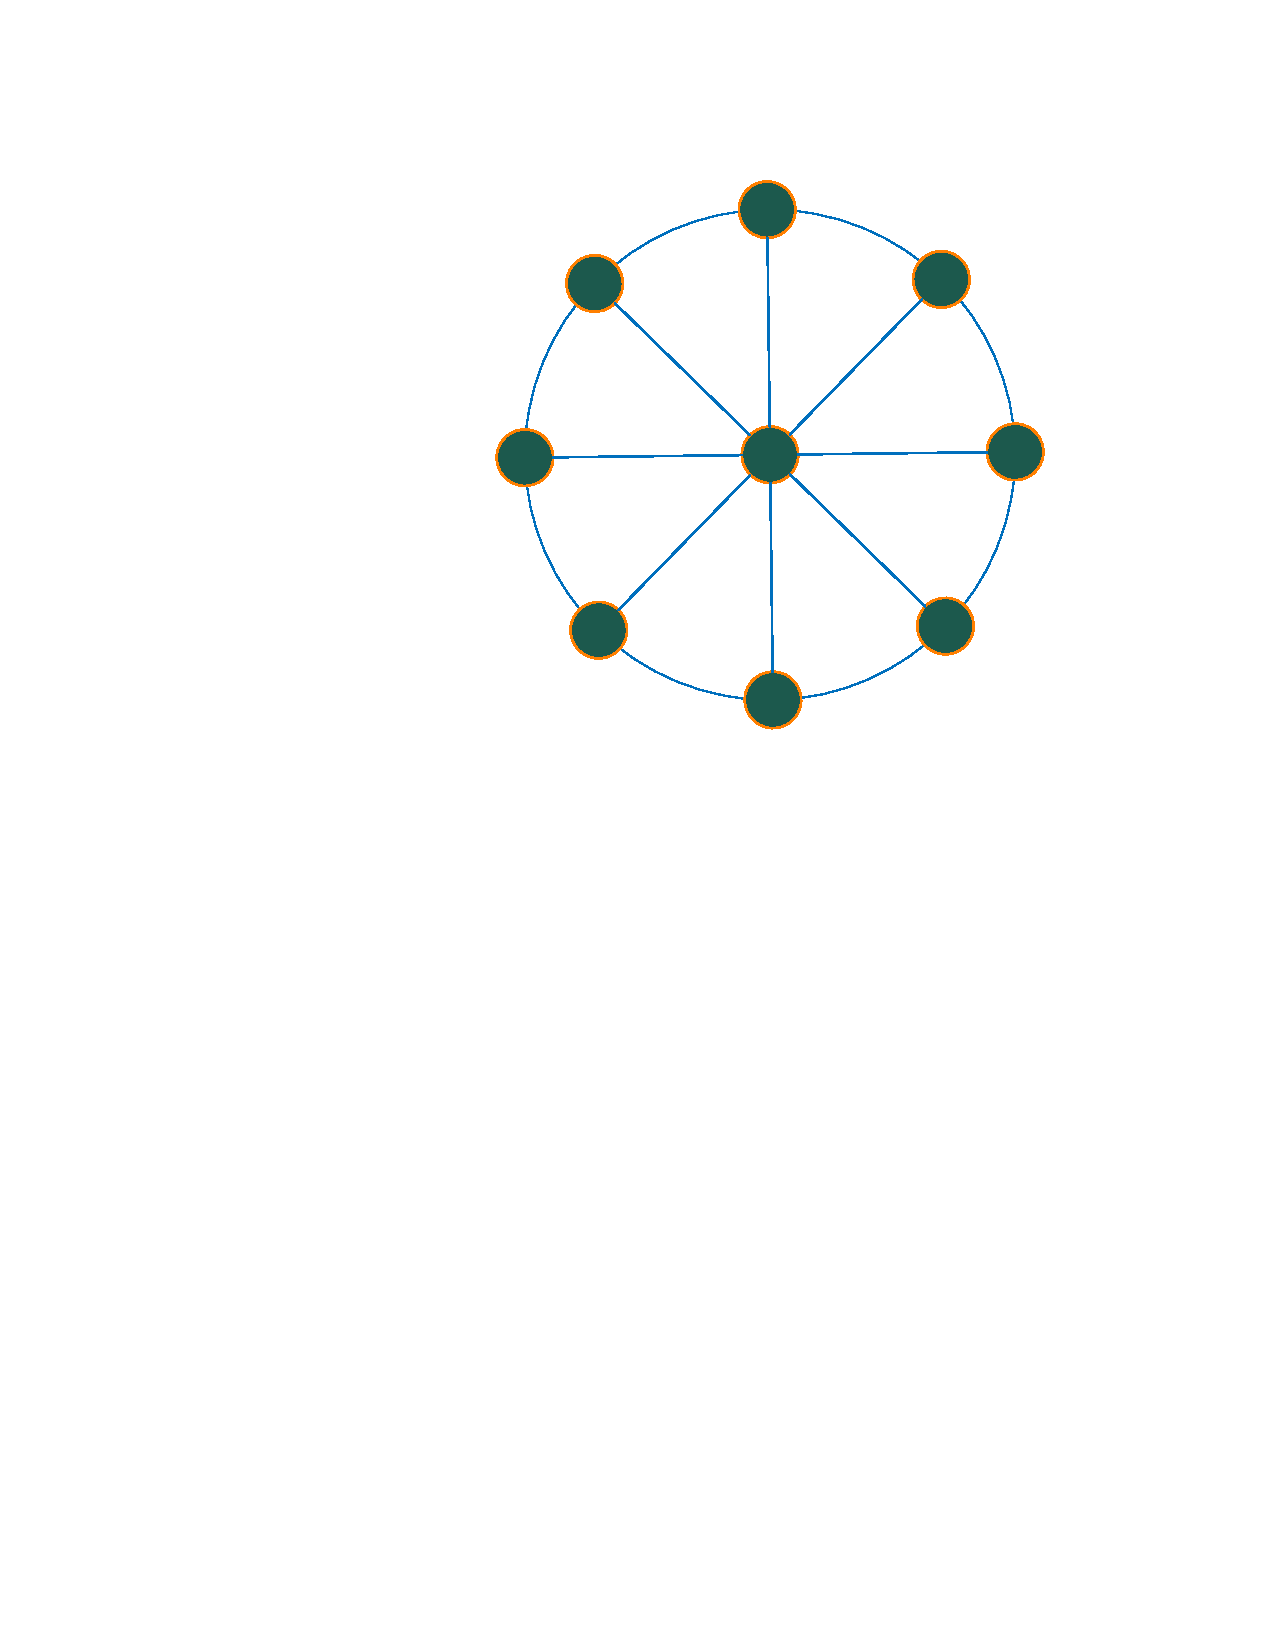
\includegraphics[width=0.68\linewidth]{P634}
		\vspace*{-5pt}
	\end{figure}
	\begin{flushright}
		\textit{Đăng Hải, Hà Nội (st)}
	\end{flushright}
	{\color{thachthuctoanhoc}{\usefont{T5}{qag}{b}{n} P635.}}
	(Mức $B$) Chứng minh rằng, với mỗi số nguyên $n\ge2$, ta luôn có:
	\begin{align*}
		\dfrac{1}{2!}+\dfrac{2}{3!}+\ldots+\dfrac{2^{n-2}}{n!}\le\dfrac{3}{2}.
	\end{align*}
	(Với mỗi số nguyên dương $k$, $k!$ (đọc là, ``$k$ giai thừa") ký hiệu tích của $k$ số nguyên dương đầu tiên; tức là, $k!=1\cdot2\cdots k$.)
	\begin{flushright}
		\textit{Lưu Bá Thắng, Hà Nội}
	\end{flushright}
	{\color{thachthuctoanhoc}{\usefont{T5}{qag}{b}{n} P636.}}
	(Mức $B$) Cho tam giác nhọn $ABC$, nội tiếp đường tròn $(O)$. Xét lục giác lồi $MNPQRS$ có các đỉnh $M, N$ thuộc cạnh $BC$, các đỉnh $P, Q$ thuộc cạnh $CA$, các đỉnh $R, S$ thuộc cạnh $AB$ sao cho
	\begin{align*}
		\angle{ROQ} &=\angle{BAC},\; \angle{MOS} =\angle{CBA}\;\\
		&\text{\color{black}và}\;\angle{NOP }= \angle{ACB}.
	\end{align*}
	Chứng minh rằng 
	\begin{align*}
		MN + PQ + RS \leq NP + QR + SM.
	\end{align*}
	\begin{figure}[H]
		\centering
		\vspace*{-5pt}
		\captionsetup{labelformat= empty, justification=centering}
		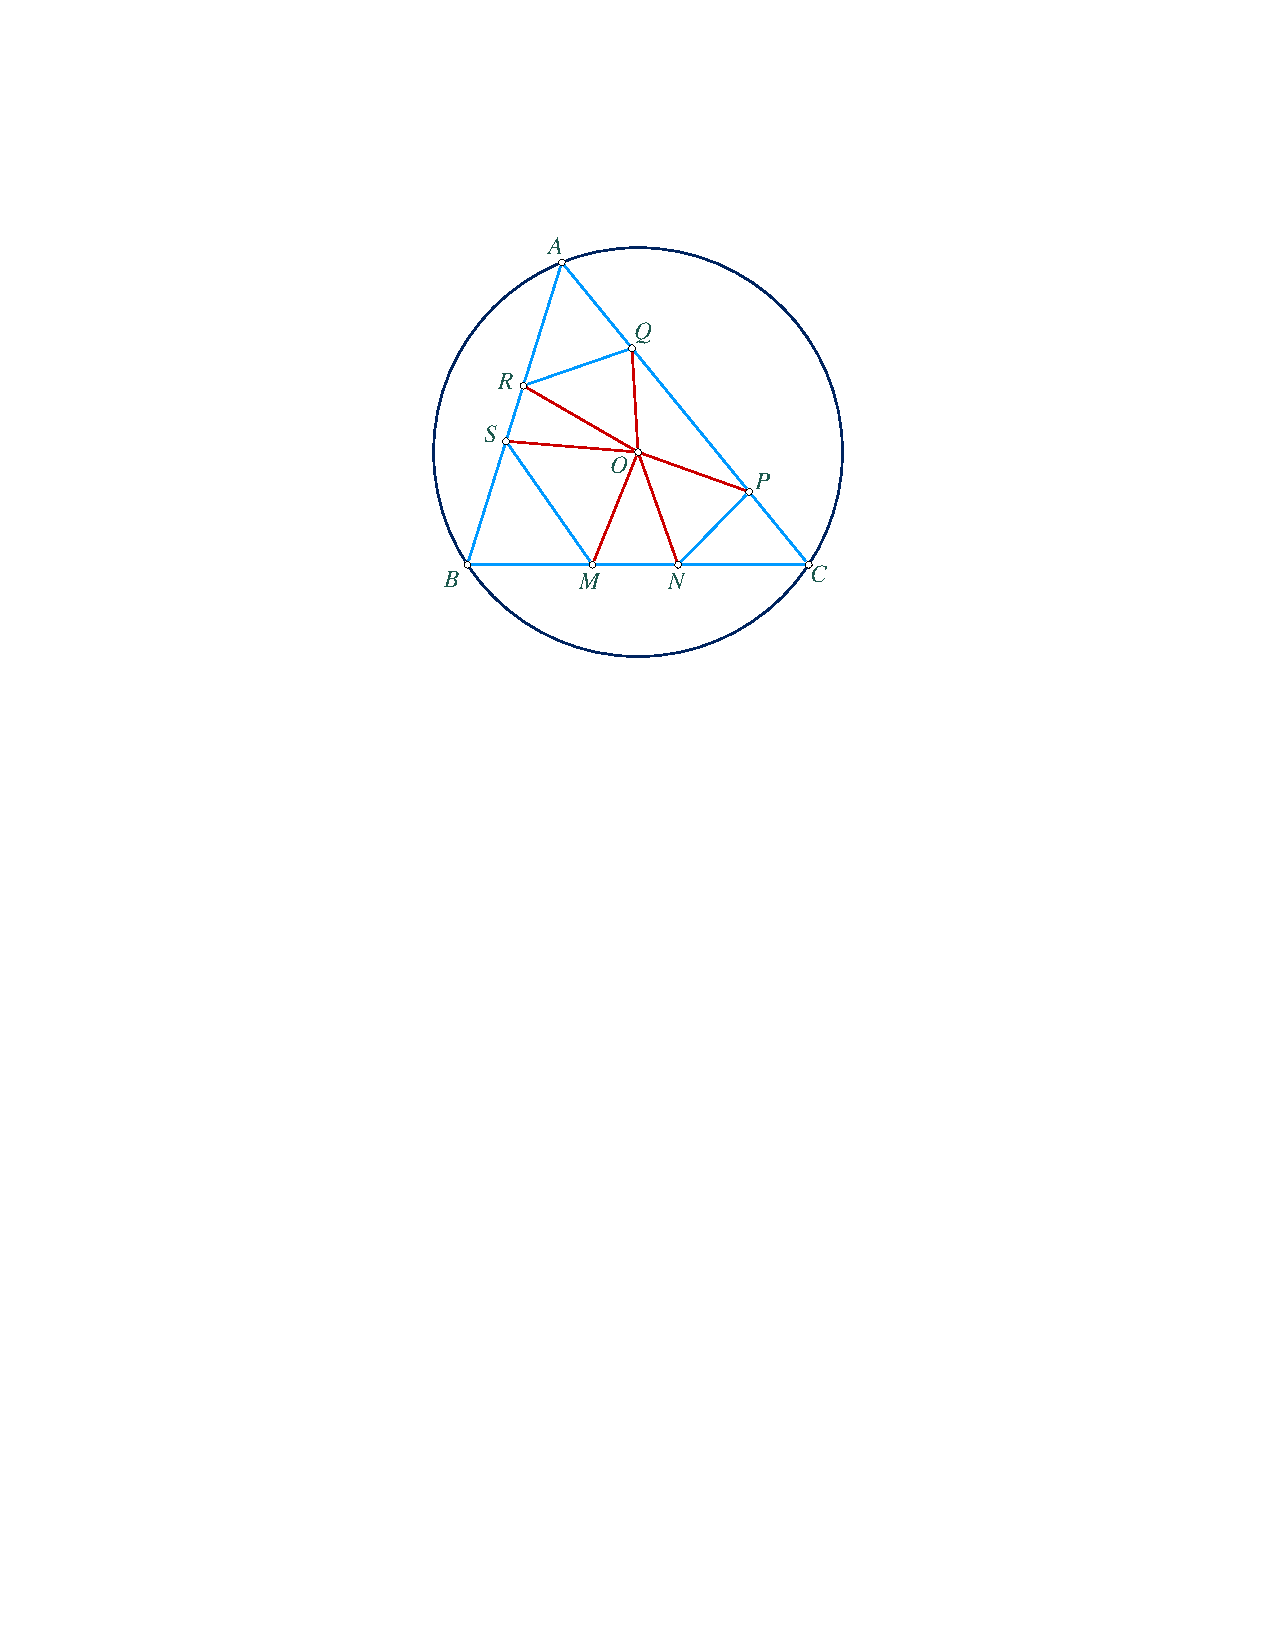
\includegraphics[width=0.7\linewidth]{P636}
		\vspace*{-5pt}
	\end{figure}
	\begin{flushright}
		\textit{Lưu Công Đông, Hà Nội}
	\end{flushright}
	{\color{thachthuctoanhoc}{\usefont{T5}{qag}{b}{n} P637.}}
	(Mức $A$) Cho số thực $a\in(0;1)$. Cho dãy số $(x_n)$, xác định bởi: $x_1=a$  và 
	\begin{align*}
		x_{n+1}=x_n\left(1-\dfrac{x_n^3+x_n^4}2\right)\quad\text{\color{black}với mọi } n\ge 1.
	\end{align*}
	Chứng minh rằng tồn tại vô số số nguyên dương $m$ sao cho 
	\begin{align*}
		\dfrac1{x_{m+1}}-\dfrac1{x_m}>\dfrac1{3\sqrt[3]{m^2}}.
	\end{align*}
	\begin{flushright}
		\textit{Nguyễn Hoàng Vinh, Đồng Nai}
	\end{flushright}
	{\color{thachthuctoanhoc}{\usefont{T5}{qag}{b}{n} P638.}}
	(Mức $A$) Tìm hai chữ số tận cùng của số $T=22^{3^{2002}}+22^{4^{2003}}$.
	\begin{flushright}
		\textit{Phạm Công Tài, Hà Nội (st)}
	\end{flushright}
	{\color{thachthuctoanhoc}{\usefont{T5}{qag}{b}{n} P639.}}
	(Mức $A$) Cho tam giác nhọn, không cân $A B C$, nội tiếp đường tròn $(O)$. Tiếp tuyến tại $B$ và $C$ của đường tròn $(O)$ cắt nhau tại $P$. Gọi $M$ là điểm chính giữa của cung $B C$ không chứa $A$ của đường tròn $(O)$. Đoạn thẳng $A M$ cắt đường tròn tâm $P$, bán kính $P B$ tại điểm $S$. Gọi $E, F$ tương ứng là hình chiếu vuông góc của $S$ trên $A C, A B$; $T, D$ tương ứng là giao điểm của $B C$ với các đường thẳng $E F$, $SO$.  Chứng minh rằng $ST \perp A D$.
	\begin{figure}[H]
		\centering
		\vspace*{-5pt}
		\captionsetup{labelformat= empty, justification=centering}
		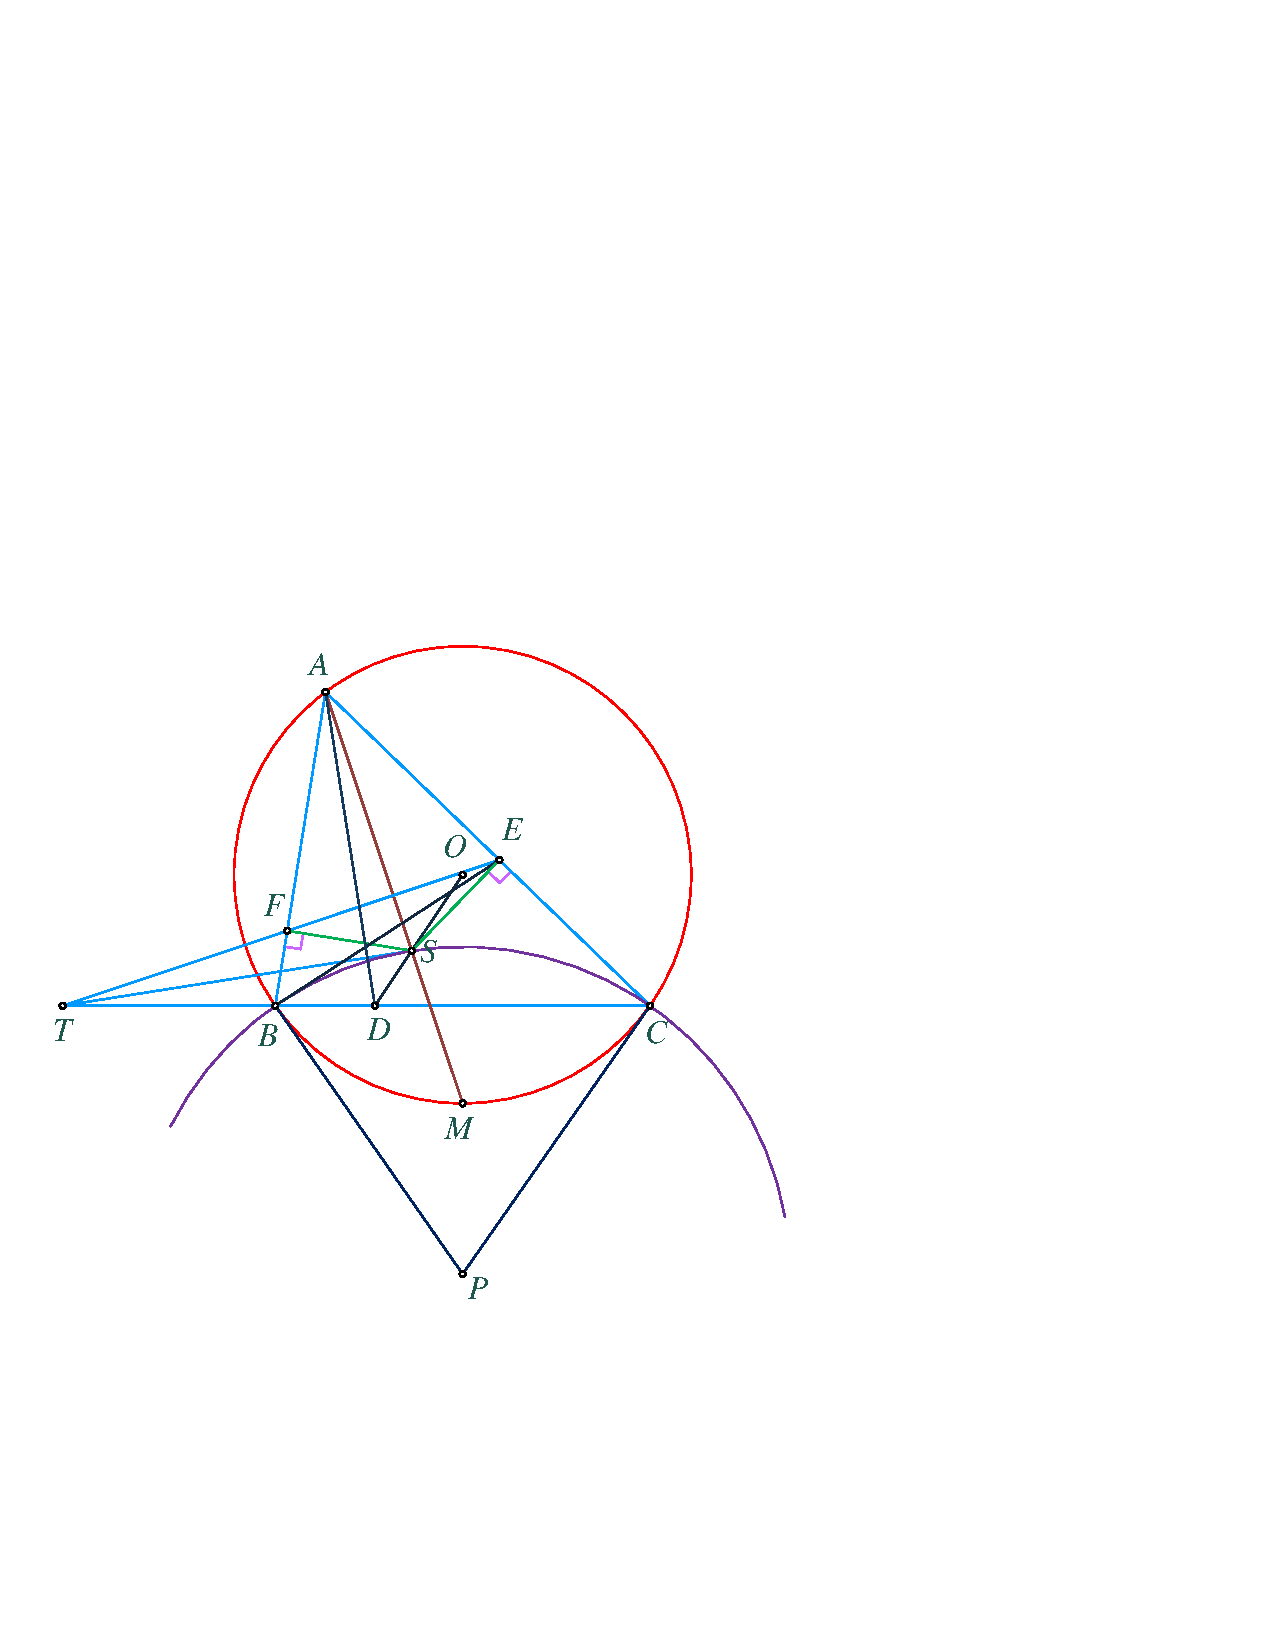
\includegraphics[width=0.85\linewidth]{P639}
		\vspace*{-10pt}
	\end{figure}
	\begin{flushright}
		\textit{Nguyễn Trường Sơn, Ninh Bình}
	\end{flushright}
	{\color{thachthuctoanhoc}{\usefont{T5}{qag}{b}{n} P640.}}
	(Mức $A$) Ký hiệu $S$ là tập hợp $2022$ số nguyên dương đầu tiên. Hỏi, có tất cả bao nhiêu tập con khác rỗng của $S$ mà tổng tất cả các số thuộc mỗi tập con đều chia hết cho $1024$?
	\vskip 0.05cm
	\hfill	\textit{Vũ Hồng Sơn, Phú Thọ}
\end{multicols}
\begin{center}
	{\large{\textbf{\color{thachthuctoanhoc}GIẢI BÀI KỲ TRƯỚC}}}
\end{center}
\begin{multicols}{2}
	\setlength{\abovedisplayskip}{4pt}
	\setlength{\belowdisplayskip}{4pt}
	{\color{thachthuctoanhoc}{\usefont{T5}{qag}{b}{n} P601.}}
	(Mức $B$) Cho bảng $3\times3$, trong đó có điền các số $1,6,12$, như ở hình dưới đây. Em hãy điền nốt vào mỗi ô chưa có số của bảng một số dương, sao cho tích ba số trong mỗi hàng, mỗi cột và mỗi đường chéo của bảng đều bằng nhau.  Hãy giải thích, em đã tìm ra các số để điền như thế nào?
	\begin{figure}[H]
		\vspace*{-5pt}
		\centering
		\begin{tikzpicture}[color=thachthuctoanhoc, scale=0.7]
			\draw (0,0) grid (3,3);
			\draw (0.5,2.5) node {$12$};
			\draw (1.5,2.5) node {$1$};
			\draw (1.5,1.5) node {$6$};
		\end{tikzpicture}
		\vspace*{-10pt}
	\end{figure}
	\textbf{\color{thachthuctoanhoc}Lời giải} (\textit{dựa theo ý giải của tất cả lời giải Tạp chí đã nhận được từ bạn đọc})\textbf{\color{thachthuctoanhoc}.}
	\vskip 0.05cm
	Ký hiệu $x$, $a$, $b$, $c$, $d$, $e$ là các số dương được điền vào các ô chưa có số của bảng đã cho, như ở hình dưới đây:
	\begin{figure}[H]
		\vspace*{-5pt}
		\centering
		\begin{tikzpicture}[color=thachthuctoanhoc, scale=0.7]
			\draw (0,0) grid (3,3);
			\draw (0.5,2.5) node {$12$};
			\draw (1.5,2.5) node {$1$};
			\draw (1.5,1.5) node {$6$};
			\draw (1.5,0.5) node {$e$};
			\draw (2.5,2.5) node {$a$};
			\draw (2.5,1.5) node {$c$};
			\draw (2.5,0.5) node {$x$};
			\draw (0.5,1.5) node {$b$};
			\draw (0.5,0.5) node {$d$};
		\end{tikzpicture}
		\vspace*{-10pt}
	\end{figure}
	Khi đó, tích các số ở mỗi hàng, mỗi cột, mỗi đường chéo chính của bảng đều bằng \linebreak$12 \cdot 6 \cdot x = 72x$.  Do đó
	\begin{align*}
		a = 72x:\left( {12 \cdot 1} \right) = 6x;
	\end{align*}
	suy ra
	\begin{align*}
		d = 72x:\left( {a \cdot 6} \right) = 72x:\left( {6x \cdot 6} \right) = 2.
	\end{align*}
	Do đó, $e = 72x:\left( {d \cdot x} \right) = 72x:\left( {2 \cdot x} \right) = 36$.
	\vskip 0.05cm
	Vì thế, từ việc xét cột thứ hai của bảng, ta được: tích các số ở mỗi hàng, mỗi cột, mỗi đường chéo chính của bảng đều bằng $1\cdot 6\cdot 36 = 216$. Suy ra
	\begin{align*}
		&x = 216:72 = 3;\,\,\, a = 6x = 6 \cdot 3 = 18;\\
		&c = 216:\left( {a \cdot x} \right) = 216:\left( {18 \cdot 3} \right) = 4;\\
		&b = 216:\left( {12 \cdot d} \right) = 216:\left( {12 \cdot 2} \right) = 9.
	\end{align*}
	Vậy, các số dương được dùng để điền vào bảng, sao cho yêu cầu của đề bài được thỏa mãn, là $18$, $9$, $4$, $2$, $36$, $3$, và chúng được điền như ở bảng ở cột bên:
	\begin{figure}[H]
%		\vspace*{-5pt}
		\centering
		\begin{tikzpicture}[color=thachthuctoanhoc, scale=0.7]
			\draw (0,0) grid (3,3);
			\draw (0.5,2.5) node {$12$};
			\draw (1.5,2.5) node {$1$};
			\draw (1.5,1.5) node {$6$};
			\draw (1.5,0.5) node {$36$};
			\draw (2.5,2.5) node {$18$};
			\draw (2.5,1.5) node {$4$};
			\draw (2.5,0.5) node {$3$};
			\draw (0.5,1.5) node {$9$};
			\draw (0.5,0.5) node {$2$};
		\end{tikzpicture}
		\vspace*{-10pt}
	\end{figure}
	\textbf{\color{thachthuctoanhoc}Bình luận và Nhận xét}
	\vskip 0.05cm
	$\pmb{1.}$ Bài đã ra là một bài toán nhẹ nhàng, ở mức bài ``Đố vui" dành cho học sinh khá, giỏi Toán lớp cuối cấp Tiểu học.
	\vskip 0.05cm
	$\pmb{2.}$ Tất cả các lời giải Tạp chí nhận được từ bạn đọc đều là lời giải đúng.
	\vskip 0.05cm
	\hfill	\textbf{\color{thachthuctoanhoc}Lê Huy}
	\vskip 0.05cm
	{\color{thachthuctoanhoc}{\usefont{T5}{qag}{b}{n} P602.}}
	(Mức $B$) Các số tự nhiên từ $1$ đến $2022$ được viết liền nhau tạo thành số $A$ dưới~đây
	\begin{align*}
		A=1234567891011\ldots 20212022.
	\end{align*}
	Nhân chữ số đầu tiên của $A$ với $2$, rồi cộng với chữ số thứ hai; nhân kết quả thu được với $2$, rồi cộng với chữ số thứ ba; tiếp theo, nhân kết quả thu được với $2$, rồi cộng với chữ số thứ tư; $\ldots$; cứ tiếp tục như thế cho đến chữ số cuối cùng của $A$. Với số mới thu được, lại làm như thế; và cứ tiếp tục làm như vậy cho đến khi thu được số có một chữ số. Hỏi, số có một chữ số thu được là số nào?
	\vskip 0.05cm
	\textbf{\color{thachthuctoanhoc}Lời giải} (\textit{dựa theo Đáp án của bài toán do Tạp chí cung cấp})\textbf{\color{thachthuctoanhoc}.}
	\vskip 0.05cm
	Để tiện cho việc diễn đạt, ta gọi toàn bộ quá trình ``nhân chữ số đầu tiên của một số tự nhiên, có ít nhất hai chữ số, với $2$, rồi cộng với chữ số thứ hai; tiếp theo, nhân kết quả thu được với $2$, rồi cộng với chữ số thứ ba; \ldots; cứ tiếp tục như thế cho đến chữ số cuối cùng của số ấy" là \textit{phép nhân -- cộng}.
	\vskip 0.05cm
	Ta có Nhận xét sau:
	\vskip 0.01cm
	\textbf{\color{thachthuctoanhoc}Nhận xét.} Sau khi thực hiện phép nhân -- cộng đối với số $N \!=\! \overline {{a_n}{a_{n - 1}} \ldots {a_1}{a_0}} $ ($n \!\in\! \mathbb{N^*}$, $n \ge 2, a_n \ne 0$) tùy ý, ta sẽ thu được số
	\begin{align*}
		N' \!=\! {a_n} \!\cdot\! {2^n} \!+\! {a_{n \!-\! 1}} \!\cdot\! {2^{n \!-\! 1}} \!+\!  \!\cdots\!  +\! {a_1} \!\cdot\! {2^1} \!+\! {a_0} \!\cdot\! {2^0}.
	\end{align*}
	Có thể dễ dàng chứng minh Nhận xét trên, bằng phương pháp quy nạp theo $n \ge 2$ (chứng minh cụ thể xin dành cho bạn đọc).
	\vskip 0.01cm
	Do
	\begin{align*}
		&{a_n} \!\cdot\! {2^n} \!+\! {a_{n - 1}} \!\cdot\! {2^{n \!-\! 1}} \!+\!  \cdots  \!+\! {a_1} \!\cdot\! {2^1} \!+\! {a_0} \!\cdot\! {2^0} \\[-0.4ex]
		< \,\,&{a_n} \cdot {10^n} + {a_{n - 1}} \cdot {10^{n - 1}} +  \cdots  \\[-0.4ex]
		&+ {a_1} \cdot {10^1} + {a_0} \cdot {10^0},
	\end{align*}
	nên từ Nhận xét suy ra, nếu $N'$  là số nguyên dương, nhận được từ số nguyên dương N nhờ phép nhân -- cộng, thì
	\begin{align*}
		N > N' > 0.
	\end{align*}
	Vì thế, trong quá trình thực hiện liên tiếp phép nhân -- cộng đối với số $A$, ta sẽ lần lượt nhận được các số nguyên dương   $A_1, A_2, \ldots$, thỏa mãn:
	\begin{align*}
		A > {A_1} > {A_2} >  \cdots  > 0.
	\end{align*}
	Từ đây, do chỉ có hữu hạn số nguyên dương thuộc nửa khoảng $(0; A]$, suy ra, quá trình thực hiện liên tiếp phép nhân -- cộng đối với số $A$ chỉ có thể gồm hữu hạn lần thực hiện phép đó. Nói một cách khác, tồn tại số nguyên dương $k$, sao cho sau $k$ lần thực hiện liên tiếp phép nhân -- cộng đối với số $A$, sẽ thu được một số tự nhiên, mà đối với nó, không thể thực hiện phép nhân -- cộng; ký hiệu số này là $A_k$.
	\vskip 0.01cm
	Từ định nghĩa phép nhân -- cộng, hiển nhiên thấy, ta không thể thực hiện phép đó đối với một số tự nhiên khi và chỉ khi số tự nhiên ấy là số có một chữ số. Do đó, $A_k$  là số có một chữ số.
	\vskip 0.01cm
	Như vậy, bằng cách thực hiện liên tiếp phép nhân -- cộng đối với số $A$, ta chắc chắn thu được một số tự nhiên có một chữ số.
	\vskip 0.01cm
	Tiếp theo, do
	\begin{align*}
			&\left({a_n} \cdot {{10}^n} + {a_{n - 1}} \cdot {{10}^{n - 1}} +  \cdots  + {a_1} \cdot {{10}^1}\right. \\[-0.4ex]
			&\left.+ {a_0} \cdot {{10}^0} \right) - \left( {a_n} \cdot {2^n} + {a_{n - 1}} \cdot {2^{n - 1}} +  \cdots\right. \\[-0.4ex]
			&\left.+ {a_1} \cdot {2^1} + {a_0} \cdot {2^0} \right)\\[-0.4ex]
			=\, &{a_n} \cdot \left( {{{10}^n} - {2^n}} \right) + {a_{n - 1}} \cdot \left( {{{10}^{n - 1}} - {2^{n - 1}}} \right) \\[-0.4ex]
			&+  \cdots + {a_1} \cdot \left( {{{10}^1} - {2^1}} \right) \equiv 0\left( {\bmod 8} \right),
	\end{align*}
	nên từ Nhận xét suy ra, nếu  $N'$ là số nguyên dương, nhận được từ số nguyên dương $N$ nhờ phép nhân -- cộng, thì
	\begin{align*}
		N \equiv N'\left( {\bmod 8} \right).
	\end{align*}
	Vì thế, ta có
	\begin{align*}
		A \equiv {A_1} \equiv {A_2} \equiv  \cdots  \equiv {A_k}\left( {\bmod 8} \right).
	\end{align*}
	Từ đó, vì
	\begin{align*}
		A &= 1234567891011 \ldots 20212 \cdot {10^3} + 22 \\[-0.4ex]
		&\equiv 22 \equiv 6\left( {\bmod 8} \right),
	\end{align*}
	nên ${A_k} \equiv 6\left( {\bmod 8} \right)$.  Mà  $A_k$ là số có một chữ số, nên $A_k = 6$.
	\vskip 0.05cm 
	Vậy, bằng cách thực hiện liên tiếp phép nhân -- cộng đối với số $A$, ta sẽ thu được một số tự nhiên có một chữ số; và số đó là $6$.
	\vskip 0.05cm
	\textbf{\color{thachthuctoanhoc}Bình luận và Nhận xét}
	\vskip 0.05cm
	$\pmb{1.}$ Trong đề bài, câu ``\textit{cứ tiếp tục làm như vậy cho đến khi thu được số có một chữ số}" chỉ thể hiện trạng thái, mà nếu gặp nó, ta sẽ kết thúc quá trình thực hiện liên tiếp phép nhân -- cộng, chứ không thể hiện trạng thái, mà ta chắc chắn sẽ thu được, sau một số hữu hạn lần thực hiện liên tiếp phép đó đối với số $A$. Hơn nữa, việc sẽ thu được hay không thể thu được một trạng thái như thế không là điều hiển nhiên, hoặc dễ thấy. Vì thế, trong lời giải của bài toán, bắt buộc phải trình bày các lập luận, khẳng định thu được hay không thể thu được số có một chữ số, nhờ việc thực hiện liên tiếp phép nhân -- cộng đối với số $A$.
	\vskip 0.05cm
	$\pmb{2.}$ Tạp chí đã nhận được $05$ (năm) lời giải, từ bạn đọc; ở tất cả các lời giải này, đều thiếu phần lập luận vừa nêu trên.
	\vskip 0.05cm
	\hfill	\textbf{\color{thachthuctoanhoc}Nguyễn Khắc Minh}
	\vskip 0.1cm
	{\color{thachthuctoanhoc}{\usefont{T5}{qag}{b}{n} P603.}}
	(Mức $B$) Lấy $n$ điểm tuỳ ý ($n\in\mathbb N^*$, $n\ge2$) nằm bên trong một hình chữ nhật kích thước  $3 \times 6$. 
	\vskip 0.05cm
	$a)$ Với $n=5$, chứng minh rằng trong các điểm đã lấy, tồn tại hai điểm mà khoảng cách giữa chúng không lớn hơn $\sqrt{10}$. 
	\vskip 0.05cm
	$b)$ Khẳng định ở câu $a)$ còn đúng không, nếu  $n=4$?
	\vskip 0.05cm
	\textbf{\color{thachthuctoanhoc}Lời giải} (\textit{của người chấm bài})\textbf{\color{thachthuctoanhoc}.}
	\vskip 0.05cm
	$a)$ Trước hết, ta nhắc lại kết quả cơ bản, quen thuộc sau:
	\vskip 0.05cm
	\textbf{\color{thachthuctoanhoc}Bổ đề.} Khoảng cách giữa hai điểm tùy ý, thuộc cùng một hình chữ nhật, không vượt quá độ dài đường chéo của hình chữ nhật ấy.
	\vskip 0.05cm
	\textit{Trở lại bài toán.}
	\vskip 0.05cm
	Chia hình chữ nhật đã cho thành hai hình vuông kích thước $3\times 3$, hình vuông màu xanh và hình vuông màu trắng, như ở Hình~$1$. Khi đó, theo nguyên lý Dirichlet, trong $5$ điểm đã lấy, tồn tại $3$ điểm cùng thuộc một hình vuông. Không mất tổng quát, giả sử $3$ điểm đó cùng thuộc hình vuông màu trắng. Chia hình vuông này thành các hình vuông đơn vị (xem Hình $2$). Khi đó, ta sẽ có một bảng ô vuông kích thước $3\times 3$ (bảng có $3$ hàng và $3$ cột).	
	\begin{figure}[H]
		\centering
		\vspace*{-10pt}
		\captionsetup{labelformat= empty, justification=centering}
		\begin{tikzpicture}[scale=0.7,color=thachthuctoanhoc]
			\filldraw [cackithi] (0,0) rectangle (3,3);
			\draw (0,0) rectangle (6,3);
			\draw (3,0) rectangle (3,3);
			\draw (7,0) grid (10,3);
		\end{tikzpicture}
		\caption{\small\textit{\color{thachthuctoanhoc}\hspace*{35pt} Hình $1$ \hspace*{70pt} Hình $2$}}
		\vspace*{-15pt}
	\end{figure}
	Xảy ra một trong hai trường hợp sau:
	\vskip 0.05cm
	$\bullet$ \textit{Trường hợp $1$: Trong ba điểm, tồn tại hai điểm thuộc cùng một hàng, hoặc cùng một cột.} Khi đó, hai điểm này sẽ thuộc một hình chữ nhật kích thước $1\times 3$, hoặc $3\times 1$. Do đó, theo Bổ đề, khoảng cách giữa chúng không vượt quá $\sqrt{3^2 + 1^2} = \sqrt{10}$.
	\vskip 0.05cm
	$\bullet$ \textit{Trường hợp $2$: Trong ba điểm, không có hai điểm nào thuộc cùng một hàng, hoặc cùng một cột.} Khi đó, ở mỗi hàng, cũng như ở mỗi cột, đều có đúng một điểm.
	\vskip 0.05cm
	Xét điểm thuộc cột $1$ và điểm thuộc cột $2$ (thứ tự của các cột được tính từ trái qua phải).
	\vskip 0.05cm
	-- \textit{Nếu hai điểm này thuộc hai hàng kề nhau} thì chúng sẽ cùng thuộc hoặc hình vuông $2\times 2$ màu hồng ở Hình $3$, hoặc hình vuông $2\times 2$ màu hồng ở Hình $4$. Bất luận thuộc hình vuông nào, khoảng cách giữa chúng, theo Bổ đề, không vượt quá
	\begin{align*}
		\sqrt {{2^2} + {2^2}}  = \sqrt 8  < \sqrt {10} .
	\end{align*}
	\begin{figure}[H]
		\centering
%		\vspace*{5pt}
		\captionsetup{labelformat= empty, justification=centering}
		\begin{tikzpicture}[scale=0.7,color=thachthuctoanhoc]
			\filldraw [toancuabi] (0,1) rectangle (2,3);
			\filldraw [toancuabi] (5,0) rectangle (7,2);
			\draw (0,0) grid (3,3);
			\draw (5,0) grid (8,3);
		\end{tikzpicture}
		\caption{\small\textit{\color{thachthuctoanhoc}Hình $3$ \hspace*{60pt} Hình $4$}}
		\vspace*{-10pt}
	\end{figure}
	-- \textit{Nếu điểm thuộc cột $1$ và điểm thuộc cột $2$ thuộc hai hàng không kề nhau} thì một điểm sẽ thuộc hàng $1$ và một điểm thuộc hàng $3$ (thứ tự của các hàng được tính từ trên xuống dưới). Do đó, điểm còn lại, trong ba điểm, sẽ thuộc ô vuông con nằm ở giao của hàng $2$ và cột $3$. Vì thế, điểm này và điểm thuộc cột $2$ cùng thuộc hoặc hoặc hình vuông $2\times 2$ màu hồng ở Hình $5$, hoặc hình vuông $2\times 2$ màu hồng ở Hình $6$. Bất luận thuộc hình vuông nào, khoảng cách giữa chúng, theo Bổ đề, không vượt quá
	\begin{align*}
		\sqrt {{2^2} + {2^2}}  = \sqrt 8  < \sqrt {10}.
	\end{align*}
	\begin{figure}[H]
		\centering
		\vspace*{-10pt}
		\captionsetup{labelformat= empty, justification=centering}
		\begin{tikzpicture}[scale=0.7,color=thachthuctoanhoc]
			\filldraw [toancuabi] (1,1) rectangle (3,3);
			\filldraw [toancuabi] (6,0) rectangle (8,2);
			\draw (0,0) grid (3,3);
			\draw (5,0) grid (8,3);
		\end{tikzpicture}
		\caption{\small\textit{\color{thachthuctoanhoc}Hình $5$ \hspace*{60pt} Hình $6.$}}
		\vspace*{-10pt}
	\end{figure}
	Kết quả xét hai trường hợp nêu trên cho thấy, trong ba điểm thuộc hình vuông $3\times 3$ màu trắng, tồn tại hai điểm có khoảng cách không vượt quá  $\sqrt{10}$. Vì thế, ta có điều phải chứng minh theo yêu cầu đề bài.
	\vskip 0.05cm
	$b)$ Xét hình chữ nhật kích thước $2,97\times 5,94$ nằm trong hình chữ nhật đã cho. Chia hình chữ nhật đó thành các hình vuông kích thước $0,99\times 0,99$, và lấy bốn điểm $A$, $B$, $C$, $D$, như ở Hình $7$. Bốn điểm này, hiển nhiên, nằm bên trong hình chữ nhật đã cho.
	\begin{figure}[H]
		\centering
		\vspace*{-10pt}
		\captionsetup{labelformat= empty, justification=centering}
		\begin{tikzpicture}[scale=0.7,color=thachthuctoanhoc]
			\draw (0,0) grid (6,3);
			\draw [fill=white] (6.,0.) circle (1.5pt);
			\draw (5.9,-0.35) node {$C$};
			\draw [fill=white] (0.,3.) circle (1.5pt);
			\draw (-0.08,3.35) node {$A$};
			\draw [fill=white] (2.,0.) circle (1.5pt);
			\draw (1.94,-0.35) node {$D$};
			\draw [fill=white] (4.,3.) circle (1.5pt);
			\draw (4.04,3.35) node {$B$};
			\draw (0,3)--(2,0) (0,3) -- (6,0) (2,0) -- (4,3) (4,3) -- (6,0);
		\end{tikzpicture}
		\caption{\small\textit{\color{thachthuctoanhoc}Hình $7$}}
		\vspace*{-5pt}
	\end{figure}
	Ta có:
	\begin{align*}
		AB &= CD = 0,99 \cdot 4 = 3,96 > \sqrt {10} .\\
		AD &= DB = BC = \sqrt {\!{{\left( {0,99 \!\cdot\! 2} \right)}^2} \!+\! {{\left( {0,99 \!\cdot\! 3} \right)}^2}}  \\
		&= 0,99 \cdot \sqrt {13}  > \sqrt {10} .\\
		AC &= \sqrt {2,{{97}^2} \!+\! 5,{{94}^2}}  = 2,97 \!\cdot\! \sqrt 5  >\! \sqrt {10}.
	\end{align*}
	Như vậy, khoảng cách giữa hai điểm bất kỳ, trong bốn điểm $A$, $B$, $C$, $D$, đều lớn hơn  $\sqrt{10}$. Vì thế, khẳng định ở câu $a)$ \textit{không} còn đúng, nếu $n = 4$.
	\vskip 0.05cm
	\textbf{\color{thachthuctoanhoc}Bình luận và Nhận xét}
	\vskip 0.05cm
	$\pmb{1.}$ Từ lời giải trên, dễ thấy, ở câu $a)$, với giả thiết ``năm điểm được lấy nằm \textit{bên trong} hình chữ nhật $3\times 6$", ta có thể chứng minh được khẳng định mạnh hơn khẳng định của đề bài. Đó là, trong năm điểm ấy, tồn tại hai điểm có khoảng cách \textit{nhỏ hơn} $\sqrt{10}$.
	\vskip 0.05cm 
	$\pmb{2.}$ Rất tiếc, tất cả các lời giải Tạp chí đã nhận được từ bạn đọc đều có lời giải câu $b)$ hoặc sai (do bốn điểm được lấy nằm trên biên của hình chữ nhật $3\times 6$, trong khi đề bài yêu cầu các điểm được lấy phải nằm bên trong hình chữ nhật đó), hoặc ``lơ mơ" (do người giải bài chỉ mô tả các điểm được lấy, mà không có bất cứ chứng cứ nào cho thấy, khoảng cách giữa hai điểm tùy ý trong các điểm ấy lớn hơn  $\sqrt{10}$).
	\vskip 0.05cm
	\hfill	\textbf{\color{thachthuctoanhoc}Hà Thanh}
	\vskip 0.05cm
	{\color{thachthuctoanhoc}{\usefont{T5}{qag}{b}{n} P604.}}
	(Mức $B$) Cho $a, b, c$ là các số thực không âm thỏa mãn $a b+b c+c a=1$. Chứng minh rằng
	\begin{align*}
		&a \sqrt{b^{2}+b c+c^{2}}+b \sqrt{c^{2}+c a+a^{2}}\\
		&+c \sqrt{a^{2}+a b+b^{2}} \le a+b+c .
	\end{align*}
	Dấu ``$=$" xảy ra khi nào?
	\vskip 0.05cm
	\textbf{\color{thachthuctoanhoc}Lời giải} (\textit{phỏng theo lời giải của các bạn Trần Đình Nam, lớp $10$T$2$, trường THPT chuyên Lê Hồng Phong, tỉnh Nam Định, và Nguyễn Chí Việt Khang, lớp $11$T$1$, trường THPT chuyên Nguyễn Quang Diêu, tỉnh Đồng Tháp})\textbf{\color{thachthuctoanhoc}.}
	\vskip 0.05cm
	Áp dụng bất đẳng thức trung bình cộng -- trung bình nhân cho hai số thực không âm  $\sqrt {{b^2} + bc + {c^2}} $ và $1$, với lưu ý tới giả thiết của đề bài, ta được:
	\begin{align*}
		&\sqrt {{b^2} + bc + {c^2}}  \le \frac{{\left( {{b^2} + bc + {c^2}} \right) + 1}}{2} \\
		= &\frac{{\left( {{b^2} + bc + {c^2}} \right) + \left( {ab + bc + ca} \right)}}{2} \\
		= &\frac{{\left( {b + c} \right)\left( {a + b + c} \right)}}{2}.
	\end{align*}
	Suy ra 
	\begin{align*}
		&a\sqrt {{b^2} + bc + {c^2}}  \\
		\le\, &\frac{{a\left( {b + c} \right)\left( {a + b + c} \right)}}{2} \quad(\text{\color{black}do } a \ge 0). \tag{$1$}
	\end{align*}
	Bằng cách hoàn toàn tương tự, ta cũng chứng minh được:
	\begin{align*}
		&b\sqrt {\!{c^2} \!+\! ca \!+\! {a^2}} \le\! \frac{{b\left( {c \!+\! a} \right)\left( {a \!+\! b \!+\! c} \right)}}{2}.\tag{$2$}\\
		&c\sqrt {\!{a^2} \!+\! ab \!+\! {b^2}} \le\! \frac{{c\left( {a \!+\! b} \right)\left(\!{a \!+\! b \!+\! c} \right)}}{2}.\tag{$3$}
	\end{align*}
	Cộng các bất đẳng thức ($1$), ($2$), ($3$), vế theo vế, ta được:
	\begin{align*}
		&a\sqrt {{b^2} + bc + {c^2}}  + b\sqrt {{c^2} + ca + {a^2}}  \\
		&+ c\sqrt {{a^2} + ab + {b^2}}  \\
		\le &\left( {ab \!+\! bc \!+\! ca} \right)\!\left( {a \!+\! b \!+\! c} \right) \!=\! a \!+\! b \!+\! c \tag{$4$}
	\end{align*}
	(do $ab + bc + ca = 1$).
	\vskip 0.05cm
	Ta có điều phải chứng minh theo yêu cầu đề bài.
	\vskip 0.05cm
	Đẳng thức ở ($4$) xảy ra khi và chỉ khi đẳng thức xảy ra đồng thời ở ($1$), ($2$) và ($3$).                    \hfill ($5$)
	\vskip 0.05cm
	Với $ab + bc + ca = 1$, ta có:
	\vskip 0.05cm
	-- Đẳng thức ở ($1$) xảy ra khi và chi khi $a = 0$, hoặc $b^2 + bc + c^2 = 1$. 
	\vskip 0.05cm 
	-- Đẳng thức ở ($2$) xảy ra khi và chi khi $b = 0$, hoặc  $c^2 + ca + a^2 = 1$.
	\vskip 0.05cm
	-- Đẳng thức ở ($3$) xảy ra khi và chi khi $c = 0$, hoặc  $a^2 + ab + b^2 = 1$.
	\vskip 0.05cm
	Vì $ab + bc + ca = 1$ nên trong ba số $a$, $b$, $c$ chỉ có thể có tối đa một số bằng $0$. Do đó, từ ($5$) và các điều kiện xảy ra đẳng thức ở ($1$), ($2$), ($3$), ta được: đẳng thức ở ($4$) xảy ra khi và chỉ khi ta có một trong các điều ($I$), ($II$), ($III$), ($IV$) sau:
	\begin{align*}
		(I)\begin{cases}
			a,b,c \ge 0\\[-0.5ex]
			ab + bc + ca = 1\\[-0.5ex] 
			a = 0\\[-0.5ex]
			{c^2} + ca + {a^2} = {a^2} + ab + {b^2} = 1.
		\end{cases}
	\end{align*}
	\begin{align*}
		(II)\begin{cases}
			a,b,c \ge 0\\[-0.5ex]
			ab + bc + ca = 1\\[-0.5ex]
			b = 0\\[-0.5ex]
			{b^2} + bc + {c^2} = {a^2} + ab + {b^2} = 1.
		\end{cases}
	\end{align*}
	\begin{align*}
		(III)\begin{cases}
			a,b,c \ge 0\\[-0.5ex]
			ab + bc + ca = 1\\[-0.5ex]
			c = 0\\[-0.5ex]
			{b^2} + bc + {c^2} = {c^2} + ca + {a^2} = 1.
		\end{cases}
	\end{align*}
	\begin{align*}
		(IV)\begin{cases}
				a,b,c \ge 0\\[-0.5ex]
				ab + bc + ca = 1\\[-0.5ex]
				abc \ne 0\\[-0.5ex]
				{b^2} + bc + {c^2} = {c^2} + ca + {a^2} \\[-0.5ex]
				\quad\quad\quad\quad\quad= {a^2} + ab + {b^2} = 1.
		\end{cases}
	\end{align*}
	Dễ thấy:
	\begin{align*}
		&(I) \Leftrightarrow a = 0 \text{ và } b = c = 1;\\[-0.5ex]
		&(II) \Leftrightarrow b = 0 \text{ và } c = a = 1;\\[-0.5ex]
		&(III) \Leftrightarrow c = 0 \text{ và } a = b = 1;\\[-0.5ex]
		&(IV) \Leftrightarrow a=b=c= \frac{1}{\sqrt{3}}.
	\end{align*}
	Vậy, dấu ``$=$" ở bất đẳng thức của đề bài xảy ra khi và chỉ khi một trong ba số $a$, $b$, $c$ bằng $0$ và hai số còn lại bằng $1$, hoặc cả ba số đó cùng bằng  $\frac{1}{\sqrt{3}}$.
	\vskip 0.05cm
	\textbf{\color{thachthuctoanhoc}Bình luận và Nhận xét}
	\vskip 0.05cm
	Tạp chí đã nhận được $10$ lời giải, từ bạn đọc. Rất tiếc, trong số này, có một lời giải sai, do người giải bài đã biến đổi sai một số biểu thức; đa phần các lời giải còn lại đều sai phần xét khả năng xảy ra dấu đẳng thức ở bất đẳng thức của đề bài, do người giải bài xử lý không đúng điều kiện xảy ra dấu đẳng thức ở bất đẳng thức Cauchy -- Bunyakovsky -- Schwarz.
	\vskip 0.05cm
	\hfill	\textbf{\color{thachthuctoanhoc}Lưu Thị Thanh Hà}
	\vskip 0.01cm
	{\color{thachthuctoanhoc}{\usefont{T5}{qag}{b}{n} P605.}}
	(Mức $B$) Cho tam giác $ABC$ cân tại $A$, có đường cao $AD$. Gọi $E$ là trung điểm $AD$; $F,G$ là hình chiếu vuông góc của $D$ trên $AC,BE$. Đường thẳng $GC$ cắt các đường thẳng $DF$ và $BF$ tương ứng tại $H$ và $I$. Chứng minh rằng $\angle{GAH}+\angle{GIF}=180^\circ$.  
	\vskip 0.05cm
	\textbf{\color{thachthuctoanhoc}Lời giải} (\textit{của người chấm bài})\textbf{\color{thachthuctoanhoc}.}
	\begin{figure}[H]
		\vspace*{-10pt}
		\centering
		\captionsetup{labelformat= empty, justification=centering}
		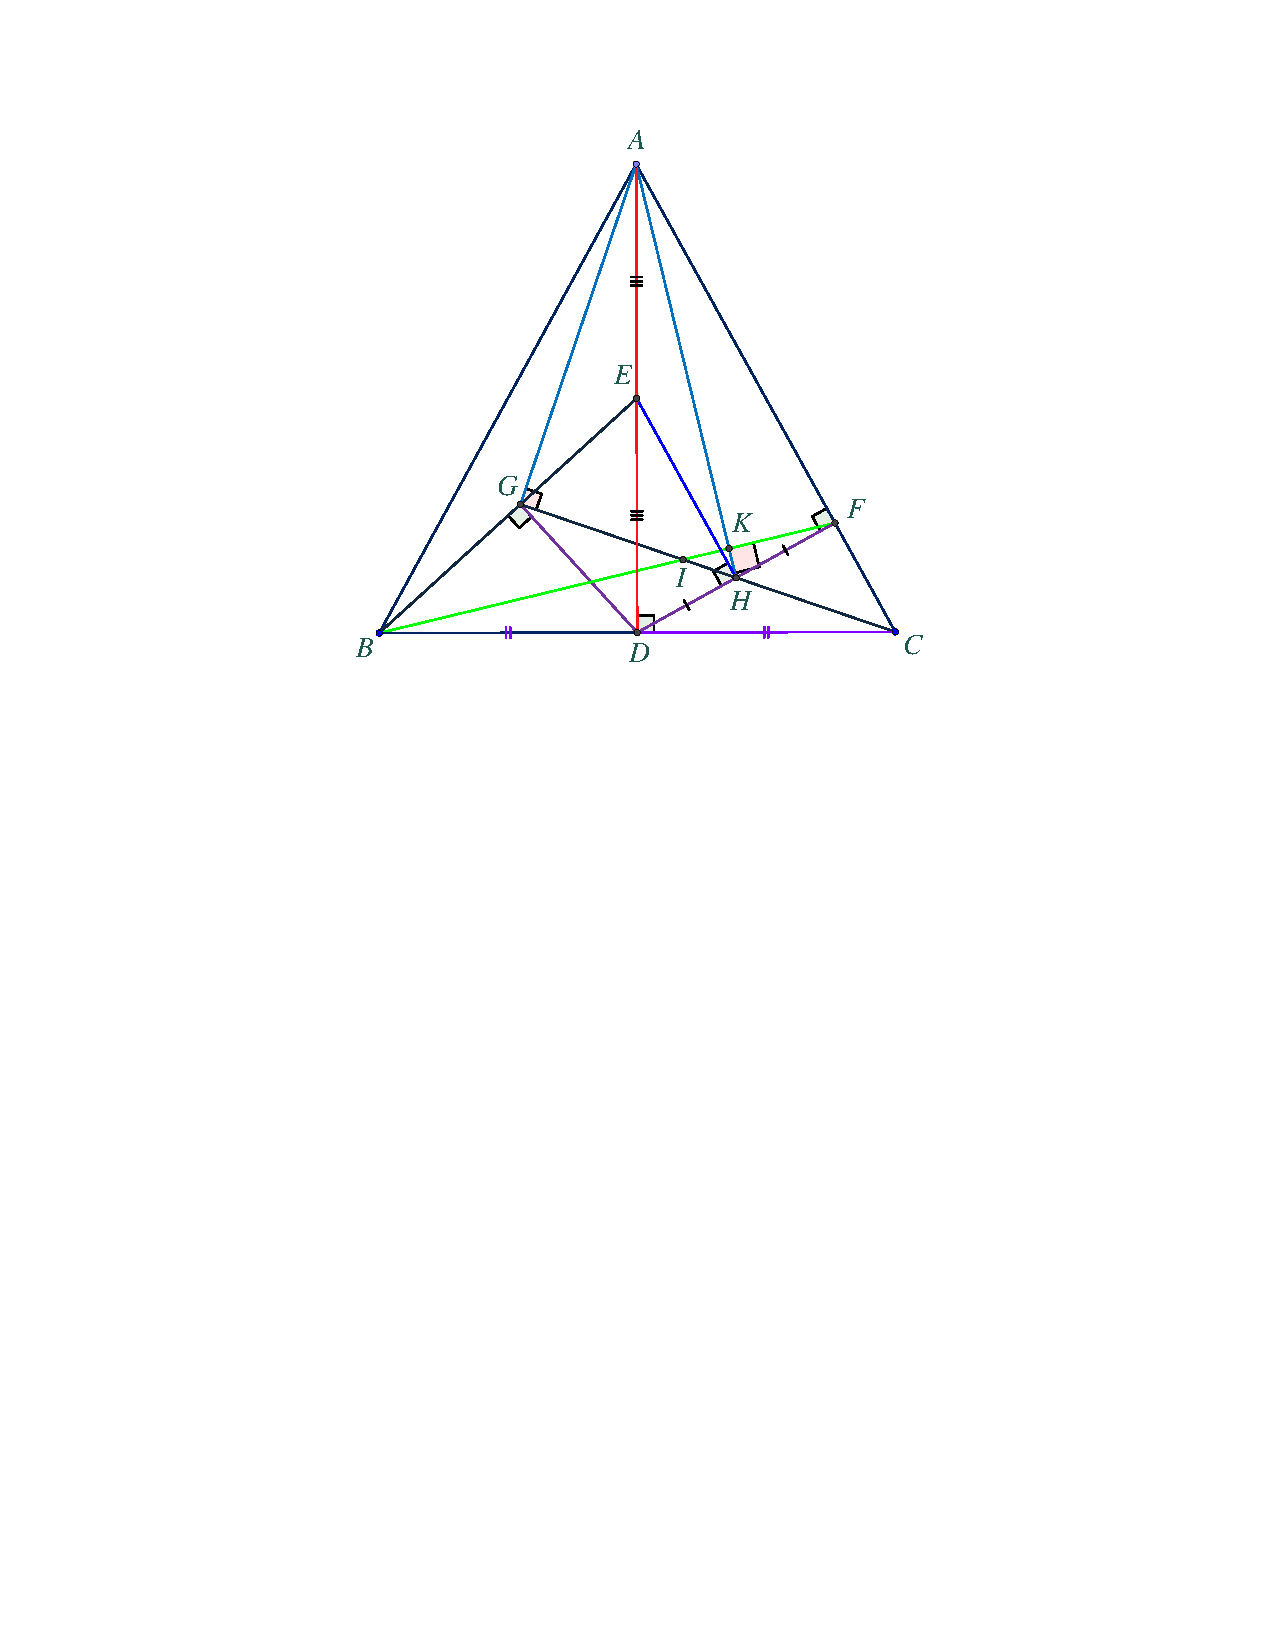
\includegraphics[width= 0.85\linewidth]{P605}
		\vspace*{-10pt}
	\end{figure}
	Gọi $K$ là giao điểm của $AH$ và $BF$. Ta sẽ chứng minh $AGIK$ là tứ giác nội tiếp.
	\vskip 0.05cm
	Do $DG \bot BE$ và $AD \bot BC$ (giả thiết), nên
	\begin{align*}
		\angle DBG = \angle EDG\tag{$1$}
	\end{align*}
	(hai góc nhọn có cạnh tương ứng vuông góc).
	\vskip 0.05cm
	Do đó, tam giác vuông $BDG$ đồng dạng với tam giác vuông $DEG$. Từ đây, vì $E$ là trung điểm của $AD$, và $D$ là trung điểm của $BC$ (do tam giác $ABC$ cân tại $A$), suy ra
	\begin{align*}
		\frac{{BC}}{{BG}} = \frac{{2BD}}{{BG}} = \frac{{2DE}}{{DG}} = \frac{{DA}}{{DG}}. \tag{$2$}
	\end{align*}
	Từ ($1$) và ($2$) suy ra,
	\begin{align*}
		\Delta GBC \sim \Delta GDA \,\,\,\text{\color{black}(c.g.c)}. \tag{$3$}
	\end{align*}
	Do đó
	\begin{align*}
		&\angle DGA = \angle BGC, \tag{$4$}\\
		&\angle DCG = \angle BCG = \angle DAG.\tag{$5$}
	\end{align*}
	Từ ($4$) suy ra
	\begin{align*}
		\angle IGA &= \angle CGA = \angle DGA - \angle DGC \\
		&= \angle BGC - \angle DGC \\
		&= \angle BGD = {90^{\circ}}. \tag{$6$}
	\end{align*}
	Từ ($5$), do $A$ và $C$ nằm cùng phía đối với $GD$, suy ra, $AGDC$ là tứ giác nội tiếp. Do đó, với lưu ý tới ($4$), ta có:
	\begin{align*}
		\angle EGH &= {180^{\circ}} - \angle BGC \\
		&= {180^{\circ}} - \angle DGA = \angle DCA. \tag{$7$}
	\end{align*}
	Do $ED \bot DC$ và $DH \bot CA$ (giả thiết), nên
	\begin{align*}
		\angle EDH = \angle DCA  \tag{$8$}
	\end{align*}
	(hai góc nhọn có cạnh tương ứng vuông góc).
	\vskip 0.05cm
	Từ ($7$) và ($8$) suy ra, $\angle EGH = \angle EDH$; do đó, $EGDH$ là tứ giác nội tiếp. Suy ra
	\begin{align*}
		\angle DHE \!=\!\! {180^{\circ}} \!-\! \angle EGD \!=\! {180^{\circ}} \!\!-\! {90^{\circ}} \!=\! {90^{\circ}}.
	\end{align*}
	Vì thế, $EH \bot DF$; suy ra, $EH \parallel AF$. Mà $E$ là trung điểm của $AD$, nên $H$ là trung điểm của $DF$. Suy ra
	\begin{align*}
		DF = 2DH.                     \tag{$9$}
	\end{align*}
	Từ ($7$) suy ra, tam giác vuông $DFA$ đồng dạng với tam giác vuông $CFD$. Do đó, với lưu ý tới ($9$), ta có:
	\begin{align*}
		\frac{{DA}}{{DH}} = \frac{{2DA}}{{DF}} = \frac{{2CD}}{{CF}} = \frac{{CB}}{{CF}}.
	\end{align*}
	Từ đây và ($8$) suy ra, $\Delta BCF \sim \Delta ADH$. Do đó
	\begin{align*}
		\angle DBK = \angle CBF = \angle DAH = \angle DAK.
	\end{align*}
	Mà $A$, $B$ nằm cùng phía đối với $DK$, nên $ABDK$ là tứ giác nội tiếp. Vì thế
	\begin{align*}
		\angle AKI = \angle AKB = \angle ADB = 90^{\circ}. \tag{$10$}
	\end{align*}
	Từ ($6$) và ($10$) suy ra, $AGIK$ là tứ giác nội tiếp. Từ đây, hiển nhiên ta có điều phải chứng minh theo yêu cầu đề bài.
	\vskip 0.05cm
	\textbf{\color{thachthuctoanhoc}Bình luận và Nhận xét}
	\vskip 0.05cm
	$\pmb{1.}$ Bài đã ra là một bài toán thú vị, rất hữu ích cho các bạn học sinh khá, giỏi toán cấp THCS, cũng như cấp THPT, trong việc rèn luyện tư duy hình học và kỹ năng giải toán hình học.
	\vskip 0.05cm
	$\pmb{2.}$ Tất cả các lời giải Tạp chí nhận được từ bạn đọc đều là lời giải đúng và hoàn chỉnh.
	\begin{flushright}
		\textbf{\color{thachthuctoanhoc}Hạ Vũ Anh}
	\end{flushright}
	{\color{thachthuctoanhoc}{\usefont{T5}{qag}{b}{n} P606.}}
	(Mức $B$) Giải hệ phương trình 
	\begin{align*}
		\begin{cases}
			\dfrac{x}{y}+\sqrt{x}&=y+\sqrt{\dfrac{y}{x}},
			\\x y+x+y&=3.
		\end{cases}
	\end{align*}
	\textbf{\color{thachthuctoanhoc}Lời giải} $\pmb{1}$ (\textit{phỏng theo ý giải của một bạn học sinh cấp THCS})\textbf{\color{thachthuctoanhoc}.}
	\vskip 0.05cm
	Điều kiện xác định của hệ phương trình: $x, y > 0$.
	\vskip 0.05cm
	$\bullet$ Dễ thấy, nếu $(x; y)$ là cặp số thực dương, mà $x \ge 3$, hoặc $y \ge 3$, thì $xy + x + y > 3$. Vì thế, trong các cặp số thực dương như vậy, không có cặp số nào là nghiệm của hệ phương trình đã cho.
	\vskip 0.05cm
	$\bullet$ Xét các cặp số thực dương $(x; y)$, mà \linebreak$0 < x, y < 3$.
	\vskip 0.05cm
	Từ phương trình thứ hai của hệ đã cho, suy ra
	\begin{align*}
		x = \frac{{3 - y}}{{y + 1}} > 0  \quad(\text{\color{black}do } 0 < y < 3).      \tag{$1.1$}
	\end{align*}
	Thế ($1.1$) vào phương trình thứ nhất của hệ đã cho, ta được:
	\begin{align*}
		\frac{{3 \!-\! y}}{{y\left( {y \!+\! 1} \right)}} \!+\! \sqrt {\frac{{3 \!-\! y}}{{y \!+\! 1}}}  \!=\! y \!+\! \sqrt {\frac{{y\left( {y \!+\! 1} \right)}}{{3 \!-\! y}}}. \tag{$1.2$}
	\end{align*}
	Vì $y \in (0; 3)$ nên
	\begin{align*}
		&\,(1.2) \\
		\Leftrightarrow &\left(\!{\frac{{3 \!-\! y}}{{{y^2} \!+\! y}} \!-\! y}\! \right) \!+\!\! \left(\!\!\!\! {\sqrt {\frac{{\left( {3 \!-\! y} \right)y}}{{{y^2} \!+\! y}}}  \!-\! \sqrt {\frac{{{y^2} \!+\! y}}{{3 \!-\! y}}} } \right) \!\!=\! 0\\
		\Leftrightarrow &\frac{{3 \!-\! y \!-\! {y^2} \!-\! {y^3}}}{{{y^2} \!+\! y}} \!+\! \frac{{\sqrt y \left( {3 \!-\! \sqrt y  \!-\! y \!-\! y\sqrt y } \right)}}{{\sqrt {{y^2} \!+\! y}  \!\cdot\! \sqrt {3 \!-\! y} }} \!=\! 0\\
		\Leftrightarrow&\frac{{\left( {1 - y} \right)\left( {3 + 2y + {y^2}} \right)}}{{{y^2} + y}} \\
		&+ \frac{{\sqrt y \left( {1 - \sqrt y } \right)\left( {3 + 2\sqrt y  + y} \right)}}{{\sqrt {{y^2} + y}  \cdot \sqrt {3 - y} }} = 0\\
		\Leftrightarrow&\left( {1 - \sqrt y } \right)\left( \frac{{\left( {1 + \sqrt y } \right)\left( {3 + 2y + {y^2}} \right)}}{{{y^2} + y}}\right. \\
		&\left.+ \frac{{\sqrt y \left( {3 + 2\sqrt y  + y} \right)}}{{\sqrt {{y^2} + y}  \cdot \sqrt {3 - y} }} \right) = 0. \tag{$1.3$}
	\end{align*}
	Do
	\begin{align*}
		&\frac{{\left( {1 + \sqrt y } \right)\left( {3 + 2y + {y^2}} \right)}}{{{y^2} + y}} \\
		&+ \frac{{\sqrt y \left( {3 + 2\sqrt y  + y} \right)}}{{\sqrt {{y^2} + y}  \cdot \sqrt {3 - y} }} > 0 \quad\forall y \in \left( {0;3} \right),
	\end{align*}
	nên: ($1.3$) $\Leftrightarrow$ $1- \sqrt{y} = 0 \Leftrightarrow y =1$. \hfill ($1.4$)   
	\vskip 0.05cm
	Thế ($1.4$) vào ($1.1$), ta được $x = 1$.
	\vskip 0.05cm
	Vì cặp số $(x; y) = (1; 1)$ nằm trong số các cặp số đang xét, và thỏa mãn điều kiện xác định, nên nó là nghiệm của hệ phương trình đã cho.
	\vskip 0.05cm
	$\bullet$ Vậy, hệ đã cho có duy nhất nghiệm $(x; y) = (1; 1)$.
	\vskip 0.05cm
	\textbf{\color{thachthuctoanhoc}Lời giải} $\pmb{2}$ (\textit{của người chấm bài})\textbf{\color{thachthuctoanhoc}.}
	\vskip 0.05cm
	Điều kiện xác định của hệ phương trình: $x, y > 0$.
	\vskip 0.05cm
	$\bullet$ Giả sử $\left( {{x_0};{y_0}} \right)$ là một nghiệm của hệ đã cho. Khi đó, ta có $x_0, y_0 > 0$  và
	\begin{align*}
		\quad\,\,\begin{cases}
			\frac{{{x_0}}}{{{y_0}}} + \sqrt {{x_0}}  = {y_0} + \sqrt {\frac{{{y_0}}}{{{x_0}}}} \quad\quad\quad\,\, &\text{\color{black}(}2.1\text{\color{black})}\\
			{x_0}{y_0} + {x_0} + {y_0} = 3.\quad\quad\quad\quad\,\, &\text{\color{black}(}2.2\text{\color{black})}
		\end{cases}
	\end{align*}
	Nhận thấy, với mọi $x, y \!\!>\!\! 0$, nếu $0 \!<\! x, y \!\!<\!\!1$\linebreak thì $xy + x + y < 3$, còn nếu $x, y > 1$ thì $xy + x + y > 3$. Vì thế, từ ($2.2$) suy ra
	\begin{align*}
		 0 < {x_0} < 1 \le {y_0}, \,\text{\color{black} hoặc }  {x_0} \ge 1 \ge {y_0} > 0.
	\end{align*}
	Tiếp theo, dễ thấy, nếu $0 < {x_0} < 1 \le {y_0}$  thì
	\begin{align*}
		\frac{{{x_0}}}{{{y_0}}} + \sqrt {{x_0}}  < 1 + 1 = 2 < {y_0} + \sqrt {\frac{{{y_0}}}{{{x_0}}}},
	\end{align*}
	mâu thuẫn với ($2.1$). Vì vậy, phải có 
	\begin{align*}
		{x_0} \ge 1 \ge {y_0} > 0. \tag{$2.3$}
	\end{align*}
	Do với mọi $x, y$ mà  $x \ge 1 \ge y > 0$, ta có
	\begin{align*}
		\frac{x}{y} + \sqrt x  \ge 1 + 1 = 2 \ge y + \sqrt {\frac{y}{x}},
	\end{align*}
	nên từ ($2.3$) suy ra
	\begin{align*}
		(2.1) &\Leftrightarrow \frac{{{x_0}}}{{{y_0}}} = \sqrt {{x_0}}  = 1 = {y_0} = \sqrt {\frac{{{y_0}}}{{{x_0}}}} \\
		&\Leftrightarrow {x_0} = {y_0} = 1.
	\end{align*}
	Như vậy, nếu $\left( {{x_0};{y_0}} \right)$ là nghiệm của hệ đã cho thì $x_0 = y_0 =1$.
	\vskip 0.05cm  
	$\bullet$ Ngược lại, bằng cách thử trực tiếp, dễ thấy cặp số $(x; y) = (1; 1)$ nghiệm đúng hệ đã cho.
	\vskip 0.05cm
	$\bullet$ Vì vậy, hệ đã cho có duy nhất nghiệm $(x; y) = (1; 1)$.
	\vskip 0.05cm
	\textbf{\color{thachthuctoanhoc}Bình luận và Nhận xét}
	\vskip 0.05cm
	Trong số các lời giải Tạp chí đã nhận được từ bạn đọc:
	\vskip 0.05cm
	-- Rất tiếc, có hai lời giải sai, gồm một lời giải sai do người giải bài đã biến đổi sai phương trình ($1.2$) trong Lời giải $1$ trên đây, và một lời giải sai do người giải bài ngộ nhận rằng, trường hợp $y \ge 1$ được xét tương tự như trường hợp $x \ge 1$. (\textit{Lưu ý các bạn, vai trò của $x$ và $y$ không như nhau trong hệ phương trình đã cho.}).
	\vskip 0.05cm
	-- Có những lời giải cho thấy, người giải bài chưa hiểu đúng về điều kiện xác định của hệ phương trình. Cụ thể, có bạn đã tìm sai điều kiện xác định của hệ phương trình, hay có bạn, sau khi nêu điều kiện xác định của hệ phương trình là ``$x, y > 0$", để giải hệ đã xét hai trường hợp, gồm trường hợp ``$y=-1$" và trường hợp ``$y \ne -1$"!
	\vskip 0.05cm
	-- Nhiều lời giải mắc lỗi không thử lại nghiệm tìm được.
	\begin{flushright}
		\textbf{\color{thachthuctoanhoc}Lưu Thị Thanh Hà}
	\end{flushright}
	{\color{thachthuctoanhoc}{\usefont{T5}{qag}{b}{n} P607.}}
	(Mức $A$) 
	Cho một nhóm có $7$ người, mà với $6$ người bất kỳ của nhóm, luôn có thể xếp họ ngồi quanh một chiếc bàn tròn, sao cho hai người ngồi cạnh nhau là hai người quen nhau. Chứng minh rằng, có thể xếp tất cả $7$ người của nhóm ngồi quanh một chiếc bàn tròn, sao cho hai người ngồi cạnh nhau là hai người quen nhau.
	\vskip 0.05cm
	\textbf{\color{thachthuctoanhoc}Lời giải} (\textit{phỏng theo ý giải của đa số lời giải Tạp chí đã nhận được từ bạn đọc})\textbf{\color{thachthuctoanhoc}.}
	\vskip 0.05cm
	Gọi nhóm $7$ người đã cho là $G$.
	\vskip 0.05cm
	Xét một người tùy ý, trong $G$; gọi người này là $X$.
	\vskip 0.05cm
	Xét $6$ người, gồm $X$ và $5$ người tùy ý trong $6$ người còn lại của $G$. Theo giả thiết, có thể xếp họ ngồi quanh một chiếc bàn tròn, sao cho hai người ngồi cạnh nhau là hai người quen nhau. Vì thế, trong $6$ người đang xét, $X$ quen ít nhất $2$ người khác, gọi là $X_1$  và $X_2$.
	\vskip 0.05cm 
	Xét $6$ người, mà trong đó không có  $X_2$. Theo giả thiết, có thể xếp họ ngồi quanh một chiếc bàn tròn, sao cho hai người ngồi cạnh nhau là hai người quen nhau. Vì thế, trong $6$ người được xét, ngoài   $X_1$, $X$ còn quen ít nhất $1$ người khác nữa.
	\vskip 0.05cm
	Như vậy, $X$ quen ít nhất $3$ người khác trong $G$. Từ đây, do $X$ là người tùy ý, nên suy ra, mỗi người trong $G$ đều quen ít nhất $3$ người khác.
	\vskip 0.05cm
	Nếu mỗi người trong $G$ đều chỉ quen đúng $3$ người khác thì số cặp quen nhau trong $G$ sẽ là
	\begin{align*}
		\dfrac{3\cdot7}{2} = 10,5 \,\,\text{\color{black} (cặp),}
	\end{align*}
	là điều vô lý (do số cặp quen nhau phải là một số tự nhiên). Vì thế, trong $G$ phải có ít nhất một người quen không ít hơn $4$ người khác.
	\vskip 0.05cm
	Xét một người bất kỳ, trong số những người quen ít nhất $4$ người khác; gọi người này là $A$.
	\vskip 0.05cm
	Theo giả thiết, có thể xếp $6$ người, mà trong đó không có $A$, ngồi quanh một chiếc bàn tròn, sao cho hai người ngồi cạnh nhau là hai người quen nhau. Ký hiệu một người tùy ý ở cách xếp này bởi  $A_1$, rồi xuất phát từ  $A_1$, lần lượt theo chiều kim đồng hồ, ký hiệu những người còn lại bởi  $A_2$,  $A_3$,  $A_4$,  $A_5$,  $A_6$. Khi đó, do $A$ quen ít nhất $4$ người, và những người này thuộc ba cặp $\left( {{A_1},{A_2}} \right)$,  $\left( {{A_3},{A_4}} \right)$,  $\left( {{A_5},{A_6}} \right)$, nên theo nguyên lý Dirichlet, phải tồn tại hai người trong số họ thuộc cùng một cặp. Xếp $A$ ngồi vào giữa hai người này, hiển nhiên ta có một cách xếp cả $7$ người ngồi quanh một chiếc bàn tròn, sao cho hai người ngồi cạnh nhau là hai người quen nhau. Khẳng định của bài ra được chứng minh.
	\vskip 0.05cm
	\textbf{\color{thachthuctoanhoc}Bình luận và Nhận xét}
	\vskip 0.05cm
	$\pmb{1.}$ Bài đã ra là một bài toán đồ thị, được phát biểu bằng ngôn ngữ đời sống. Bằng ngôn ngữ của Lý thuyết đồ thị, bài toán được phát biểu như sau:
	\vskip 0.05cm
	``\textit{Cho $G$ là một đồ thị đơn, vô hướng, $7$ đỉnh, và có tính chất: mỗi đồ thị con $6$ đỉnh của $G$ là một đồ thị Hamilton. Chứng minh rằng, $G$ là đồ thị Hamilton.}"
	\vskip 0.05cm
	(Trong một số tài liệu, khái niệm ``đồ thị con" trong phát biểu trên được gọi là ``đồ thị con cảm sinh".)
	\vskip 0.05cm
	$\pmb{2.}$ Lời giải trên đây sẽ trở nên ngắn gọn và đỡ ``rườm rà" câu chữ hơn nhiều, nếu diễn đạt bằng ngôn ngữ của Lý thuyết đồ thị. Tuy nhiên, để tiện lợi cho tất cả các đối tượng bạn đọc trong việc theo dõi lời giải, chúng tôi đã không lựa chọn phương án diễn đạt\linebreak vừa nêu.
	\vskip 0.05cm
	$\pmb{3.}$ Dưới đây là một trong những phương án khái quát của bài đã ra:
	\vskip 0.05cm
	\textbf{\color{thachthuctoanhoc}Một phương án khái quát.} Cho số nguyên dương $n$, và cho một nhóm có $2n + 1$ người, mà với $2n$ người bất kỳ của nhóm, luôn có thể xếp họ ngồi quanh một chiếc bàn tròn, sao cho hai người ngồi cạnh nhau là hai người quen nhau. Khi đó, ta có thể xếp tất cả $2n + 1$ người của nhóm ngồi quanh một chiếc bàn tròn, sao cho hai người ngồi cạnh nhau là hai người quen nhau.
	\vskip 0.05cm
	\textit{Một câu hỏi dành cho bạn đọc: Khẳng định ở phương án khái quát nêu trên đúng hay sai?}
	\vskip 0.05cm
	$\pmb{4.}$ Rất tiếc, trong số các lời giải Tạp chí đã nhận được từ bạn đọc, có hai lời giải sai, gồm một lời giải sai do người giải bài chưa xét hết các trường hợp có thể xảy ra, và một lời giải sai do người giải bài đã có những ngộ nhận trong lập luận (vì những ngộ nhận này mà bạn đọc đó đã khẳng định trường hợp ``mỗi người trong nhóm $7$ người quen đúng ba người khác" có thể xảy ra, và đã chỉ ra cách xếp $7$ người ngồi quanh bàn tròn, thỏa mãn yêu cầu đề bài, trong trường hợp đó). Bên cạnh hai lời giải sai vừa nêu, có một lời giải không hoàn chỉnh, do người giải bài đã sử dụng sai khái niệm chu trình Hamilton trong các lập luận.
	\vskip 0.05cm
	$\pmb{5.}$ Sử dụng phương pháp phản chứng để tiếp cận các bài toán với yêu cầu ``chứng minh tồn tại" là một cách tiếp cận tự nhiên. Tuy nhiên, với bài đã ra, nếu giải bằng phương pháp phản chứng, thì giả sử phản chứng chỉ được dùng để triệt tiêu những thông tin hữu ích, giúp đi thẳng đến đích, sau khi đã khai thác được những thông tin đó chỉ từ các giả thiết của bài toán. Vì thế, lời giải bằng phương pháp phản chứng cho bài đã ra sẽ là một lời giải ``vòng vo", rối rắm.
	\begin{flushright}
		\textbf{\color{thachthuctoanhoc}Nguyễn Khắc Minh}
	\end{flushright}	
	{\color{thachthuctoanhoc}{\usefont{T5}{qag}{b}{n} P608.}}
	(Mức $A$) Xét các số thực $a,b,c$ thuộc đoạn $[0;1]$ và thoả mãn $a+b+c=2$. Hãy xác định giá trị lớn nhất của biểu thức
	\begin{align*}
		P=a^4+b^4+c^4+\dfrac{11}2abc.
	\end{align*}
	\textbf{\color{thachthuctoanhoc}Lời giải} (\textit{dựa theo Đáp án do Tạp chí cung cấp})\textbf{\color{thachthuctoanhoc}.}
	\vskip 0.05cm
	Trước hết, ta có Nhận xét sau:
	\vskip 0.05cm
	\textbf{\color{thachthuctoanhoc}Nhận xét.} Với mọi $x \in [0;1]$,  ta có:
	\begin{align*}
		{x^4} \le \frac{{11{x^2} - 9x + 2}}{4}
	\end{align*}
	\textit{Chứng minh.} Do $x \in [0;1]$  nên
	\begin{align*}
		{\left( {2x - 1} \right)^2}\left( {x - 1} \right)\left( {x + 2} \right) \le 0. \tag{$1$}
	\end{align*}
	Ta có:
	\begin{align*}
		(1) \Leftrightarrow &\left( {4{x^2} - 4x + 1} \right)\left( {{x^2} + x - 2} \right) \le 0\\
		\Leftrightarrow &\,\, 4{x^4} - 11{x^2} + 9x - 2 \le 0\\
		\Leftrightarrow & \,\,{x^4} \le \frac{{11{x^2} - 9x + 2}}{4}.
	\end{align*}
	Nhận xét được chứng minh.
	\vskip 0.05cm
	Do $a,b,c \in [0;1]$ nên áp dụng Nhận xét lần lượt cho $x = a$, $x = b$, $x = c$, rồi cộng ba bất đẳng thức thu được, vế theo vế, ta được:
	\begin{align*}
			&{a^4} + {b^4} + {c^4} \\
			\le &\frac{{11\left( {{a^2} + {b^2} + {c^2}} \right) - 9\left( {a + b + c} \right) + 6}}{4}\\
			 = &\frac{{11}}{2}\!\left( {2 \!-\! \left( {ab \!+\! bc \!+\! ca} \right)\!} \right) \!-\! 3\left({{\text{\color{black}do }}a \!+\! b \!+\! c \!=\!\! 2} \right)\\
			 = &\,8 - \frac{{11}}{2}\left( {ab + bc + ca} \right).
	\end{align*}
	Suy ra
	\begin{align*}
		P \le 8 - \frac{{11}}{2}\left( {ab + bc + ca - abc} \right).\tag{$2$}
	\end{align*}
	Tiếp theo, do  $a,b,c \in [0;1]$ nên
	\begin{align*}
			&ab + bc + ca - abc\\
			 = &\left( {1 \!- \!a} \right)\left( {1 \!-\! b} \right)\left( {1 \!-\! c} \right) \!+\! \left( {a \!+\! b \!+\! c} \right) \!-\! 1\\
			= &\left( {1 \!-\! a} \right)\left( {1 \!-\! b} \right)\left( {1 \!-\! c} \right) \!+\! 1\left( {{\text{\color{black}do }}a \!+\! b \!+\! c \!=\! 2} \right)\\
			\ge &1. \tag{$3$}
	\end{align*}
	Từ ($2$) và ($3$), suy ra
	\begin{align*}
		P \le 8 - \frac{{11}}{2} \cdot 1 = \frac{5}{2}.
	\end{align*}
	Hơn nữa, với $a = 1$ và $b = c   = \frac{1}{2}$  ta có $a + b + c = 2$ và  $P = \frac{5}{2}$.
	\vskip 0.05cm 
	Vì vậy, giá trị lớn nhất của $P$ bằng $\frac{5}{2}$.
	\vskip 0.05cm  
	\textbf{\color{thachthuctoanhoc}Bình luận và Nhận xét}
	\vskip 0.05cm
	$\pmb{1.}$ Chìa khóa để giải bài đã ra là Nhận xét ở Lời giải trên. Theo người chấm bài, rất rất khó để nhìn ra chiếc chìa khóa đó.
	\vskip 0.05cm
	$\pmb{2.}$ Rất tiếc, tất cả các lời giải Tạp chí nhận được từ bạn đọc đều là lời giải sai, do người giải bài đã mắc ít nhất một trong các \linebreak lỗi sau:
	\vskip 0.05cm
	-- Cho rằng, $P$ là một hàm số của biến $a$, với $b$, $c$ là các tham số;
	\vskip 0.05cm
	-- Cho rằng, với  $a,b \!\in\! [0;1]$, nếu $a \!+\! b \!+\! c \!\!=\!\! 2$ thì  $2\sqrt[4]{{\dfrac{{{a^4} + {b^4}}}{2}}} + c = 2$;
	\vskip 0.05cm
	(\textit{Phản ví dụ cho khẳng định vừa nêu trên}: \linebreak $a = \dfrac{1}{3}, b = \dfrac{2}{3}$, và $c = 1$.)
	\vskip 0.05cm
	-- Thực hiện sai các biến đổi và đánh giá.
	\begin{flushright}
		\textbf{\color{thachthuctoanhoc}Lê Huy}
	\end{flushright}
	{\color{thachthuctoanhoc}{\usefont{T5}{qag}{b}{n} P609.}}
	(Mức $A$) Cho tam giác $ABC$, có đường cao $AD$ $(D\in BC)$. Hai điểm $E,F$ nằm trên cạnh $BC$ sao cho $\angle{BAE}=\angle{CAF}$. Lấy điểm $K$ bất kỳ trên $AD$. Gọi $Y$ và $Z$ tương ứng là hình chiếu vuông góc của $A$ trên $KE$ và $KF$. Chứng minh rằng đường tròn ngoại tiếp tam giác $DYZ$ tiếp xúc với đường tròn Euler của tam giác $ABC$.
	\vskip 0.05cm
	\textbf{\color{thachthuctoanhoc}Lời giải} (\textit{dựa theo Đáp án do Tạp chí cung cấp})\textbf{\color{thachthuctoanhoc}.}
	\vskip 0.05cm
	Gọi $O$, $J$ và $L$ tương ứng là tâm đường tròn ngoại tiếp, tâm đường tròn Euler của tam giác $ABC$ và tâm đường tròn ngoại tiếp tam giác $DYZ$.
	\vskip 0.05cm
	Gọi $H$ là trực tâm tam giác $ABC$; ta có, $J$ là trung điểm của $HO$.\hfill       ($1$)
	\vskip 0.05cm
	Gọi $P$ là điểm đối xứng với $A$ qua $J$; ta có, $AHPO$ là hình bình hành (do ($1$)). Suy ra, $AH \parallel OP$ và $AH = OP$. Do đó, $OP \bot BC$ (vì $AH \bot BC$) và $OP$ bằng hai lần khoảng cách từ $O$ đến $BC$ (vì $AH$ bằng hai lần khoảng cách từ $O$ đến $BC$). Vì thế, $O$ và $P$ đối xứng với nhau qua $BC$.\hfill              ($2$)
	\begin{figure}[H]
		\vspace*{-10pt}
		\centering
		\captionsetup{labelformat= empty, justification=centering}
		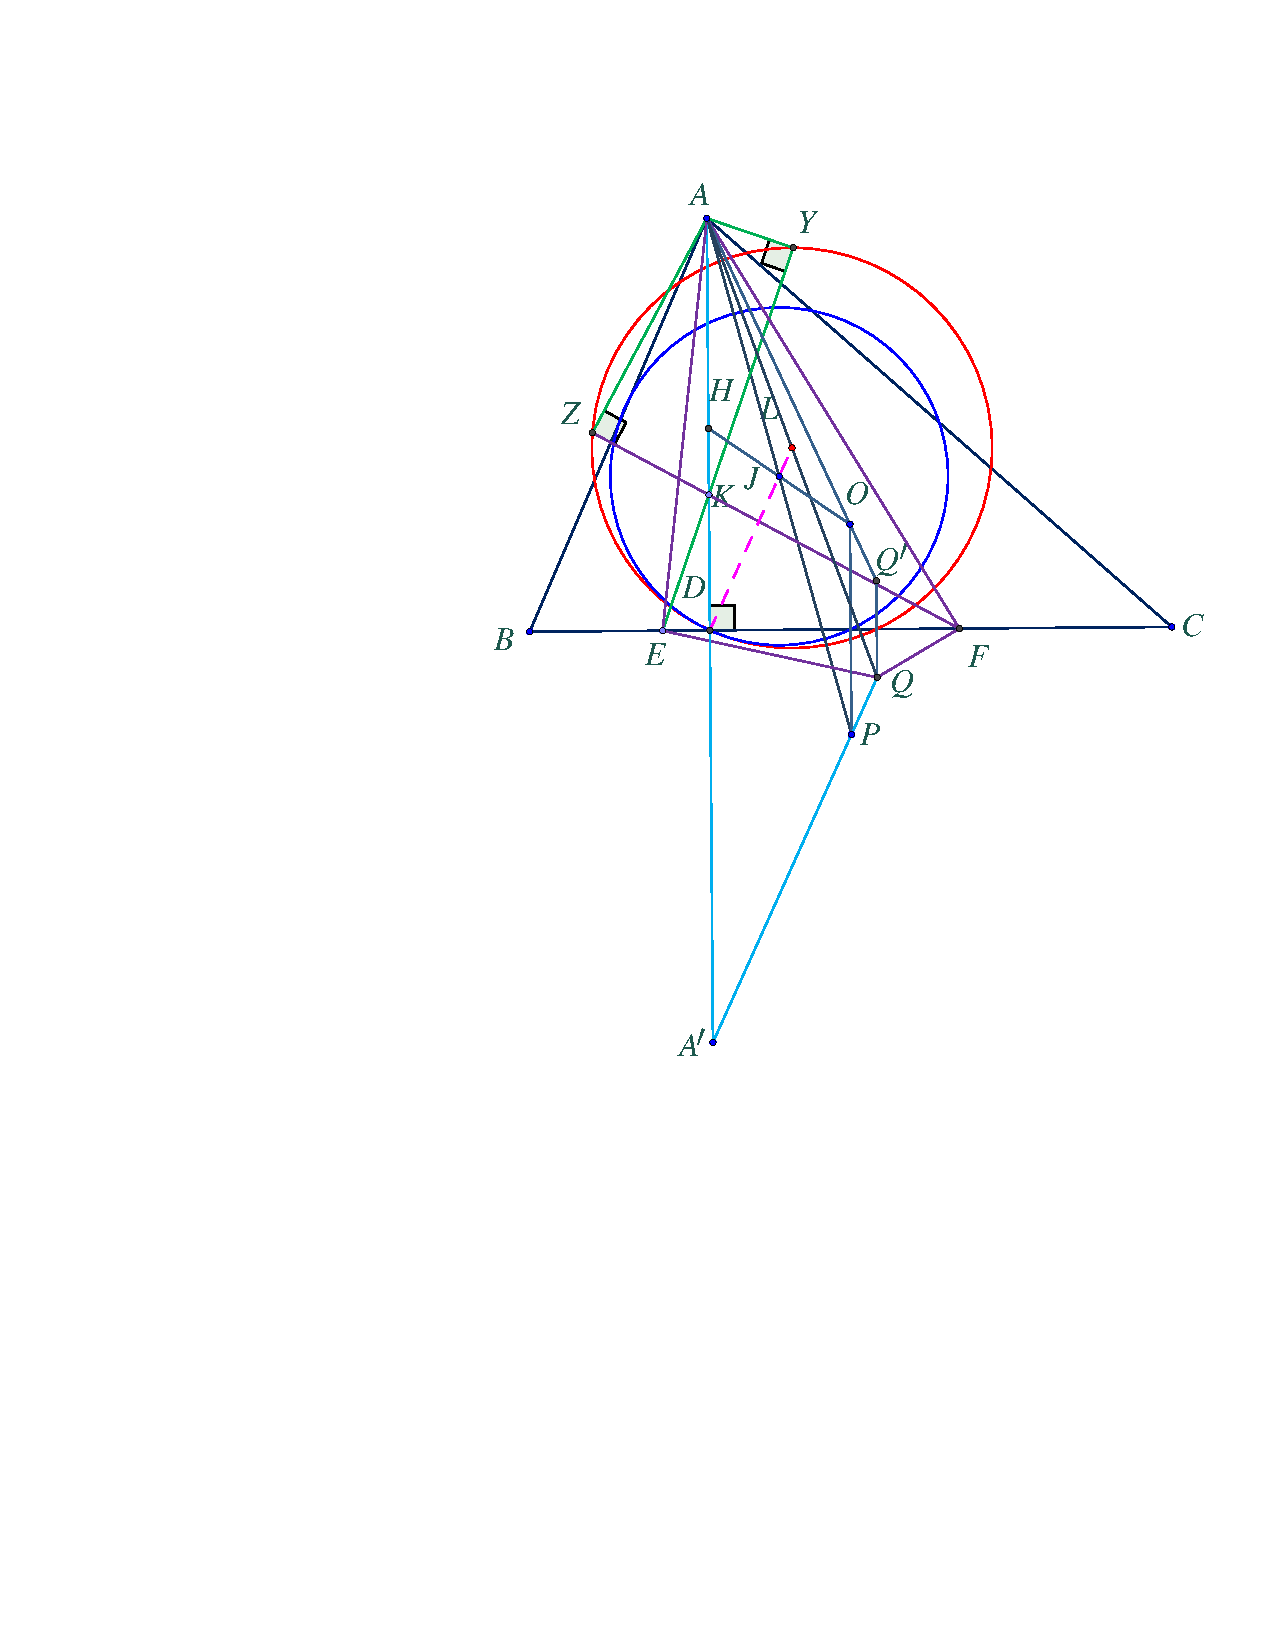
\includegraphics[width= 1\linewidth]{P609}
		\vspace*{-15pt}
	\end{figure}
	Gọi $Q$ là điểm liên hợp đẳng giác của $A$ đối với tam giác $KEF$; ta có:
	\vskip 0.05cm
	-- $L$ là trung điểm của $AQ$; \hfill ($3$)
	\vskip 0.05cm
	-- $EQ$, $EA$ đẳng giác đối với $\angle KEF$ và $FQ$, $FA$ đẳng giác đối với      $\angle KFE$.\hfill    ($4$)
	\vskip 0.05cm
	Gọi  $A',Q'$ tương ứng là điểm đối xứng với $A$, $Q$ qua $BC$. Khi đó, với lưu ý tới ($4$), ta có:
	\begin{align*}
		&\angle Q'EF = \angle FEQ = \angle KEA \\
		\text{\color{black}và } &\angle Q'FE = \angle EFQ = \angle KFA.
	\end{align*}
	Suy ra, $EQ', EK$ đẳng giác đối với $\angle AEF$, và $FQ', FK$ đẳng giác đối với $\angle EFA$. Do đó, $K$, $Q'$ liên hợp đẳng giác đối với tam giác $AEF$. Vì thế, $AK$, $AQ'$ đẳng giác đối với $\angle EAF$.  Mà $AE$, $AF$ đẳng giác đối với $\angle BAC$,  nên $AK$, $AQ'$ đẳng giác đối với $\angle BAC$. Từ đây, do $AH$, $AO$ đẳng giác đối với $\angle BAC$, và $K \in  AH$, nên  $Q' \in AO$; nói cách khác, $A$, $O$, $Q'$ là ba điểm thẳng hàng. Mà  $A'$, $P$, $Q$ tương ứng đối xứng với $A$, $O$, $Q'$ qua $BC$ (theo ($2$) và định nghĩa các điểm  $A'$, $Q'$), nên ba điểm  $A'$, $P$, $Q$  thẳng hàng. Từ đây, do $L$, $J$, $D$ tương ứng là trung điểm của $AQ$, $AP$, $AA'$ (theo ($3$) và định nghĩa các điểm $P$,  $A'$), nên $L$, $J$, $D$ là ba điểm thẳng hàng. Vì thế, từ $D$ là điểm chung của đường tròn ngoại tiếp tam giác $DYZ$ và đường tròn Euler của tam giác $ABC$, và $L$, $J$ là tâm của hai đường tròn đó, suy ra, hai đường tròn này tiếp xúc với nhau. Ta có điều phải chứng minh theo yêu cầu đề bài.
	\vskip 0.05cm
	\textbf{\color{thachthuctoanhoc}Bình luận và Nhận xét}
	\vskip 0.05cm
	$\pmb{1.}$ Bài đã ra là một bài toán thú vị, xoay quanh các tính chất của hai đường đẳng giác đối với một góc, và của cặp điểm liên hợp đẳng giác đối với một tam giác.
	\vskip 0.05cm
	$\pmb{2.}$ Dễ thấy, $\overline {KD}  \cdot \overline {KA}  = \overline {KY}  \cdot \overline {KE}  = \overline {KZ}  \cdot \overline {KF}$. Vì thế, ký hiệu $k$ là giá trị chung của ba tích vừa nêu, ta có, phép nghịch đảo $I_K^k$  biến $A$ thành $D$, $E$ thành $Y$, và $F$ thành $Z$. Do đó, có thể chứng minh khẳng định của bài ra bằng cách dựa vào một đường tròn tiếp xúc với đường tròn $(AEF)$ tại $A$, mà qua phép nghịch đảo $I_K^k$, đường tròn này biến thành đường tròn Euler của tam giác $ABC$.
	\vskip 0.05cm
	$\pmb{3.}$ Một số lời giải, trong số các lời giải mà Tạp chí nhận được từ bạn đọc, đã mắc một trong các lỗi sau:
	\vskip 0.05cm
	-- Viết nhầm lẫn tên các điểm;
	\vskip 0.05cm
	-- Sử dụng các ký hiệu không có trong Toán học, nhưng không giải thích (ví dụ, ký hiệu $\overline {X,Y,Z} ,$ với $X$, $Y$, $Z$ là các điểm);
	\vskip 0.05cm
	-- Diễn giải sai phép nghịch đảo.
	\vskip 0.05cm
	Tất cả các lời giải mắc một trong các lỗi nêu trên không được coi là lời giải hoàn chỉnh.
	\vskip 0.05cm
	\hfill	\textbf{\color{thachthuctoanhoc}Hạ Vũ Anh}
	\vskip 0.05cm
	{\color{thachthuctoanhoc}{\usefont{T5}{qag}{b}{n} P610.}}
	(Mức $A$) Tìm tất cả các hàm số \linebreak $f: \mathbb{R} \rightarrow \mathbb{R}$ thỏa mãn
	\begin{align*}
		f(x f(x)+y)=f(y)+x^{2}
	\end{align*}
	với mọi $x,y\in\mathbb R$.
	\vskip 0.05cm
	\textbf{\color{thachthuctoanhoc}Lời giải} (\textit{của người chấm bài})\textbf{\color{thachthuctoanhoc}.}
	\vskip 0.05cm
	$\bullet$ Giả sử $f: \mathbb{R} \to \mathbb{R}$ là một hàm số thỏa mãn yêu cầu đề bài; nghĩa là, ta có:
	\begin{align*}
		f\left( {x \cdot f\left( x \right) + y} \right) = f\left( y \right) + {x^2}, \tag{$1$}
	\end{align*}
	với mọi  $x,y \in \mathbb{R}$.
	\vskip 0.05cm
	Lần lượt thế $y = 0$, và $y = -x \cdot f(x)$  vào ($1$), ta được:
	\begin{align*}
		&f\left( {x \cdot f\left( x \right)} \right) = f\left( 0 \right) + {x^2}, \tag{$2$}\\
		&f\left( { - x \cdot f\left( x \right)} \right) = f\left( 0 \right) - {x^2},
	\end{align*}
	với mọi  $x \in \mathbb{R}$. Suy ra, $f$  là một toàn ánh từ $\mathbb{R}$  đến  $\mathbb{R}$. Do đó, tồn tại số thực $a$, sao cho $f(a )= 0$.
	\vskip 0.05cm 
	Thế $x = a$ vào ($2$), ta được
	\begin{align*}
		f\left( 0 \right) = f\left( 0 \right) + {a^2};
	\end{align*}
	do đó, $a = 0$. Như vậy,  $f(0) = 0$; vì thế, theo ($2$), ta có:
	\begin{align*}
		f\left( {x \cdot f\left( x \right)} \right) = {x^2}, \tag{$3$}
	\end{align*}
	với mọi  $x \in \mathbb{R}$.
	\vskip 0.05cm
	Thế $x = 1$ vào ($3$), ta được:  $f\left( {f\left( 1 \right)} \right) = 1;$ do đó, thế  $x = f(1)$ vào ($3$), ta được:
	\begin{align*}
		{\left( {f(1)} \right)^2} \!=\! f\left( {f(1) \cdot f\left( {f(1)} \right)} \right) \!=\! f\left( {f(1)} \right) \!=\! 1.
	\end{align*}
	Suy ra, $f(1) = 1$ hoặc $f(1) = -1$.
	\vskip 0.05cm  
	$\diamond$ \textit{Trường hợp} $1$: $f(1) = 1$.
	\vskip 0.05cm  
	Khi đó, thế $x = 1$ vào ($1$), ta được:
	\begin{align*}
		f\left( {y + 1} \right) = f\left( y \right) + 1,
	\end{align*}
	với mọi  $y \in \mathbb{R}$.
	\vskip 0.05cm
	Do đó, trong ($1$), thay $x$ bởi $x + 1$, ta được:
	\begin{align*}
		&{\left( {x + 1} \right)^2} + f\left( y \right) \\
		= &f\left( {\left( {x + 1} \right) \cdot f\left( {x + 1} \right) + y} \right) \\
		= &f\left( {\left( {x + 1} \right) \cdot \left( {f\left( x \right) + 1} \right) + y} \right)\\
		=& f\left( {x \cdot f\left( x \right) + f\left( x \right) + x + y + 1} \right)\quad\quad\quad\quad\\
		=& f\left( {x \cdot f\left( x \right) + f\left( x \right) + x + y} \right)\\
		&+ 1, \quad\forall x, y \in \mathbb{R}.\tag{$4$}
	\end{align*}
	Trong ($1$), thay $y$ bởi $f(x) + x +y$,  ta được:
	\begin{align*}
		&f\left( {x \cdot f\left( x \right) + f\left( x \right) + x + y} \right)\\
		= &f\left( {f\left( x \right) + x + y} \right) + {x^2}, \quad\forall x,y \in \mathbb{R}. \tag{$5$}
	\end{align*}
	Từ ($4$) và ($5$), ta có:
	\begin{align*}
			&{\left( {x + 1} \right)^2} + f\left( y \right) \\
			= &f\left( {f\left( x \right) + x + y} \right) + {x^2} + 1, \quad \forall x,y \in \mathbb{R}.
	\end{align*}
	Suy ra
	\begin{align*}
		f\left( {f\left( x \right) + x + y} \right) = 2x + f\left( y \right), \tag{$6$}
	\end{align*}
	với mọi $x,y \in \mathbb{R}$.
	\vskip 0.05cm
	Tiếp theo, giả sử $u, v$ là hai số thực sao cho $f(u) = f(v)$. Khi đó, theo ($6$), ta có:
	\begin{align*}
		&2u + f\left( v \right) = f\left( {f\left( u \right) + u + v} \right) \\
		= &f\left( {f\left( v \right) \!+\! u \!+\! v} \right) \!=\! 2v +\! f\left( u \right) \!=\! 2v +\! f\left( v \right);
	\end{align*}
	suy ra, $u = v$. Vì thế, $f: \mathbb{R} \to \mathbb{R}$ là một đơn ánh.
	\vskip 0.05cm
	Trong ($6$), thay $x$ bởi $\dfrac{f(x)}{2}$  và $y = 0$, với lưu ý $f(0)=0$,  ta được:
	\begin{align*}
		f\left( {f\left( {\frac{{f\left( x \right)}}{2}} \right) + \frac{{f\left( x \right)}}{2}} \right) = f\left( x \right), \quad\forall x \in \mathbb{R}.
	\end{align*}
	Mà $f$ là đơn ánh, nên
	\begin{align*}
		f\left( {\frac{{f\left( x \right)}}{2}} \right) + \frac{{f\left( x \right)}}{2} = x, \quad\forall x \in \mathbb{R}.
	\end{align*}
	Do đó, trong ($6$), thay $x$ bởi  $\dfrac{f(x)}{2}$, ta được:
	\begin{align*}
		f\left( {x + y} \right) = f\left( x \right) + f\left( y \right), \quad\forall x,y \in \mathbb{R}.
	\end{align*}
	Vì thế, $f$  là một hàm cộng tính.
	\vskip 0.05cm
	Thế $y = 0$ vào ($6$), ta được:
	\begin{align*}
		f\left( {f\left( x \right) + x} \right) = 2x, \quad\forall x \in \mathbb{R}. \tag{$7$}
	\end{align*}
	Do đó, trong ($3$), thay $x$ bởi $x + f(x)$  với lưu ý $f$  là hàm cộng tính, ta có:
	\begin{align*}
			&{\left( {x + f\left( x \right)} \right)^2} \\
			= &f\left( {\left( {x + f\left( x \right)} \right) \cdot f\left( {x + f\left( x \right)} \right)} \right) \\
			= &f\left( {\left( {x + f\left( x \right)} \right) \cdot 2x} \right)\\
			= &f\left(\! {2{x^2} \!+\! 2x \!\cdot\! f\left( x \right)} \!\right)\\ =& 2f\!\left(\! {{x^2}} \right) \!+\! 2f\left( {x \!\cdot\! f\left( x \right)} \right)\\
			= &2\left( {f\left( {{x^2}} \right) + {x^2}} \right),\quad \forall x\in \mathbb{R}. \tag{$8$}
	\end{align*}
	Trong ($7$), thay $x$ bởi $x \cdot f(x)$  và sử dụng ($3$), ta có:
	\begin{align*}
		2x \cdot f\left( x \right) &= f\left( {f\left( {x \cdot f\left( x \right)} \right) + x \cdot f\left( x \right)} \right) \\[-0.4ex]
		&= f\left( {{x^2} + x \cdot f\left( x \right)} \right)\\[-0.4ex]
		&= f\left( {{x^2}} \right) + f\left( {x \cdot f\left( x \right)} \right) \\[-0.4ex]
		&= f\left( {{x^2}} \right) + {x^2}, \quad\forall x\in \mathbb{R}. \tag{$9$}
	\end{align*}
	Từ ($8$) và ($9$), suy ra
	\begin{align*}
		{\left( {x + f\left( x \right)} \right)^2} = 4x \cdot f\left( x \right),\quad\forall x \in \mathbb{R}.
	\end{align*}
	Do đó,  ${\left( {x - f\left( x \right)} \right)^2} = 0,\,\forall x\in \mathbb{R}$. Suy ra  
	\begin{align*}
		f(x) = x, \forall x \in \mathbb{R}.
	\end{align*}
	$\diamond$ \textit{Trường hợp} $2$: $f(1) = -1$.
	\vskip 0.05cm  
	Thế $x = 1$ vào ($3$), ta được $f\left( {f\left( 1 \right)} \right) = 1;$  do đó, $f(-1) = 1$.
	\vskip 0.05cm 
	Xét hàm số  $g: \mathbb{R} \to \mathbb{R}$, xác định bởi \linebreak$g(x) = f(-x)$, với mọi $x \in \mathbb{R}$. Ta có:
	\begin{align*}
		g\left( {x \cdot g\left( x \right) + y} \right) &= f\left( { - x \cdot f\left( { - x} \right) - y} \right) \\[-0.4ex]
		&= f\left( { - y} \right) + {\left( { - x} \right)^2} \\[-0.4ex]
		&= g\left( y \right) + {x^2},\quad\forall x,y \in \mathbb{R}.
	\end{align*}
	Như thế, $g$ là một hàm số thỏa mãn yêu cầu đề bài, và có $g(1) = f(-1) = 1$. Do đó, theo kết quả xét trường hợp $1$, ta có  $g(x) \!=\! x$, \linebreak$\forall x\in \mathbb{R}$. Suy ra,  $f(x) = -x, \forall x \in \mathbb{R}$.
	\vskip 0.05cm
	Như vậy, nếu $f$  là hàm số thỏa mãn yêu cầu đề bài thì  $f(x) = x, \forall x \in \mathbb{R}$, hoặc  $f(x) = -x$, $\forall x \in \mathbb{R}$.
	\vskip 0.05cm
	$\bullet$ Ngược lại, bằng phép thử trực tiếp, dễ thấy, hai hàm số vừa nêu trên thỏa mãn yêu cầu đề bài. Vì thế, chúng là tất cả các hàm số cần tìm theo yêu cầu đề bài.
	\vskip 0.05cm
	\textbf{\color{thachthuctoanhoc}Bình luận và Nhận xét}
	\vskip 0.05cm
	$\pmb{1.}$ Phải chăng, bài đã ra là một mở rộng của một bài toán trong Đề thi Olympic Toán học châu Âu dành cho học sinh nữ (EGMO) năm $2021$, bằng cách thay tập $\mathbb{Q}$  bởi tập  $\mathbb{R}$?
	\vskip 0.05cm
	\textbf{\color{thachthuctoanhoc}Bài toán trong Đề thi EGMO $\pmb{2021}$.} \textit{Tìm tất cả các hàm số $f: \mathbb{Q} \to \mathbb{Q}$, thỏa mãn
	\begin{align*}
		f\left( {x \cdot f\left( x \right) + y} \right) = f\left( y \right) + {x^2},
	\end{align*}
	với mọi  $x, y \in \mathbb{Q}$.}
	\vskip 0.05cm
	$\pmb{2.}$ Ở bài đã ra, nếu thay tập $\mathbb{R}$  bởi tập $\mathbb{R^+}$  (tập các số thực dương), ta sẽ thu được một bài toán cũng rất thú vị. Và từ bài toán này, ta thu được kết quả khái quát sau:
	\vskip 0.05cm
	\textbf{\color{thachthuctoanhoc}Bài toán khái quát.} \textit{Cho $f,g,h: \mathbb{R^+} \to \mathbb{R^+}$  là các hàm số thỏa mãn
	\begin{align*}
		f\left( {g\left( x \right) + y} \right) = h\left( x \right) + f\left( y \right),
	\end{align*}
	với mọi $x,y \in \mathbb{R^+}$. Chứng minh rằng, hàm số  $\dfrac{g(x)}{h(x)}$ là một hàm hằng.}
	\vskip 0.05cm
	$\pmb{3.}$ Rất tiếc, trong các lời giải Tạp chí đã nhận được từ bạn đọc, có một lời giải sai, do người giải bài đã mắc một số lỗi chuyên môn; chẳng hạn, từ  $(f(x))^2 \!=\! {x^2},\forall x \!\in\! \mathbb{R}$, suy ra  $f(x) \!=\! x$, $\forall x \in \mathbb{R}$, hoặc  $f\left( x \right) =  - x,\forall x \in \mathbb{R}$.
	\vskip 0.05cm
	\hfill	\textbf{\color{thachthuctoanhoc}Võ Quốc Bá Cẩn}
\end{multicols}
\begin{center}
	\textbf{\color{thachthuctoanhoc}DANH SÁCH HỌC SINH CÓ LỜI GIẢI HOÀN CHỈNH}
\end{center}
\textit{Trong các ngoặc đơn ở phần dưới đây, sau tên lớp là mã hiệu của các bài toán mà học sinh có lời giải hoàn chỉnh.}
\begin{multicols}{2}
	\textbf{\color{thachthuctoanhoc}KHỐI THCS}
	\vskip 0.05cm
	$\bullet$ Trường \textbf{\color{thachthuctoanhoc}THCS xã Pom Lót}, huyện Điện Biên, tỉnh Điện Biên: \textit{Nguyễn Ngọc Diệp} (lớp $8$C$3$; P$601$).
	\vskip 0.05cm
	$\bullet$ Trường \textbf{\color{thachthuctoanhoc}THPT chuyên Hà Nội -- Amsterđam}, Tp. Hà Nội: \textit{Hà Mạnh Hùng} (lớp $7$A; P$601$, P$607$).
	\vskip 0.05cm
	$\bullet$ Trường \textbf{\color{thachthuctoanhoc}THCS Việt Nam -- Angiêri}, Tp. Hà Nội: \textit{Vương Khánh Toàn} (lớp $9$A$1$; P$601$, P$605$).
	\vskip 0.05cm
	$\bullet$ Trường \textbf{\color{thachthuctoanhoc}THCS Nguyễn Trãi}, huyện Đại Lộc, tỉnh Quảng Nam: \textit{Nguyễn Châu Tuấn Kiệt} (lớp $9/7$; P$605$, P$606$).
	\vskip 0.05cm
	\textbf{\color{thachthuctoanhoc}KHỐI THPT}
	\vskip 0.05cm
	$\bullet$ Trường \textbf{\color{thachthuctoanhoc}THPT số $\pmb{2}$ Phù Cát}, tỉnh Bình Định: \textit{Nguyễn Hữu Trí} (lớp $10$A$1$; P$605$).
	\vskip 0.05cm
	$\bullet$ Trường \textbf{\color{thachthuctoanhoc}THPT chuyên Nguyễn Quang Diêu}, tỉnh Đồng Tháp: \textit{Hoàng Nguyễn Gia Bảo} (lớp $10$T$1$; P$601$), \textit{Nguyễn Chí Việt Khang} (lớp $11$T$1$; P$601$, P$604$, P$605$), \textit{Đỗ Duy Quang} (lớp $10$T$1$; P$601$), \textit{Phạm Hồng Thanh Thảo} (lớp $10$T$1$; P$601$).
	\vskip 0.05cm
	$\bullet$ Trường \textbf{\color{thachthuctoanhoc}THPT Gia Định}, Tp. Hồ Chí Minh: \textit{Lê Anh Khoa} (lớp $10$CT; P$605$), \textit{Nguyễn Hà Ngọc Uyên} (lớp $11$CT; P$601$, P$605$).
	\vskip 0.05cm
	$\bullet$ Trường \textbf{\color{thachthuctoanhoc}THPT chuyên Hưng Yên}, tỉnh Hưng Yên: \textit{Trần Hữu Dương} (lớp $10$ Toán $1$; P$601$, P$606$), \textit{Nguyễn Gia Khánh} (lớp $10$ Toán $1$; P$609$).
	\vskip 0.05cm
	$\bullet$ Trường \textbf{\color{thachthuctoanhoc}THPT chuyên Thăng Long}, tỉnh Lâm Đồng: \textit{Thân Ngô Tuấn} (lớp $10$ Toán; P$601$).
	\vskip 0.05cm
	$\bullet$ Trường \textbf{\color{thachthuctoanhoc}THPT chuyên Lê Hồng Phong}, tỉnh Nam Định: \textit{Ngô Quang Bình} (lớp $10$T$1$; P$601$), \textit{Trần Đình Nam} (lớp $10$T$2$; P$601$, P$604$).
	\vskip 0.05cm
	$\bullet$ Trường \textbf{\color{thachthuctoanhoc}THPT chuyên Hoàng Lê Kha}, tỉnh Tây Ninh: \textit{Thái Gia Huy} (lớp $11$T; P$609$).
	\vskip 0.05cm
	$\bullet$ Trường \textbf{\color{thachthuctoanhoc}THPT chuyên Quốc học Huế}, tỉnh Thừa Thiên -- Huế: \textit{Nguyễn Chính Minh} (lớp $10$ Toán $1$; P$605$, P$610$), \textit{Nguyễn Đình Khải Nguyên} (lớp $11$ Toán $2$; P$601$), \textit{Đỗ Đại Phong} (lớp $10$ Toán $1$; P$605$), \textit{Nguyễn Thị Nhật Thảo} (lớp $11$ Toán $2$; P$601$, P$605$), \textit{Trần Thị Thanh Thư} (lớp $11$ Toán $1$; P$601$), \textit{Đặng Quỳnh Bảo Uyên} (lớp $11$ Toán $2$; P$601$).
	\vskip 0.05cm
	$\bullet$ Trường \textbf{\color{thachthuctoanhoc}THPT chuyên Khoa học tự nhiên}, ĐH Khoa học tự nhiên -- ĐHQG Hà Nội: \textit{Mai Quốc Anh} (lớp $11$A$2$ Toán; P$607$).
	\vskip 0.05cm
	$\bullet$ Trường \textbf{\color{thachthuctoanhoc}THPT chuyên Sư phạm}, ĐH Sư phạm Hà Nội: \textit{Hồ Trần Khánh Linh} (lớp $11$ Toán $2$; P$607$).
\end{multicols}
\vspace*{-10pt}
\rule{1\linewidth}{0.1pt}
\begin{center}
	\textbf{\LARGE\color{thachthuctoanhoc}LỜI GIẢI, ĐÁP ÁN}
\end{center}

\begin{multicols}{2}
	\textbf{\color{thachthuctoanhoc}Quấy rầy thám tử}
	\vskip 0.05cm
	Vinh và Sinh không thể cùng nói dối, như vậy trong số họ phải có một người nói thật. Vì thế Du phải là người nói dối, khi khẳng định rằng cậu ta không làm vỡ kính. Vậy người làm vỡ kính là Du.
	\vskip 0.05cm
	\textbf{\color{thachthuctoanhoc}Đố vui}
	\vskip 0.05cm
	Đánh số các quả cân từ $1$ đến $6$. 
	\vskip 0.05cm
	Trước hết cân $1$ với $2$. Giả sử chúng nặng bằng nhau. Ở lần cân thứ hai, ta cân $1$ với $3$. Nếu chúng nặng bằng nhau thì $1$, $2$, $3$ là các quả cân nặng bằng nhau (cũng như $4$, $5$ và $6$). Do đó ở lần cân thứ $3$ ta chỉ cần so sánh $1$ và $4$ để xác định được những quả cân nào là đúng và những quả cân nào là sai. Nếu không, chẳng hạn $1$ nặng hơn $3$ (trường hợp $1$ nhẹ hơn $3$ tương tự), thì các quả cân $1$ và $2$ là các quả cân đúng và quả cân $3$ là quả cân sai. Bây giờ, trong số các quả cân $4$, $5$, $6$ có một quả cân đúng và hai quả cân sai. Để xác định, ta chỉ cần cân $4$ với $5$: nếu chúng nặng bằng nhau thì nghĩa là $4$ chúng là các quả cân sai; nếu không, quả nặng hơn là quả cân đúng (còn hai quả còn lại là quả cân sai). 
	\vskip 0.05cm
	Bây giờ, giả sử $1$ nặng hơn $2$ (trường hợp ngược lại tương tự), nghĩa là quả cân $1$ là đúng và quả cân $2$ là sai. Ở lần cân thứ hai, ta cân $1$ với $3$ để xác định được $3$ là quả cân đúng hai sai. Như vậy, sau $2$ lần cân, ta xác định được ba quả cân $1$, $2$, $3$: gồm hai quả đúng và một quả sai hoặc hai quả sai và một quả đúng. Ở lần cân cuối cùng, ta tiến hành như ở trường hợp bên trên, bằng cách cân $4$ với $5$, để xác định được những quả cân nào đúng và quả cân nào sai.  
	\vskip 0.05cm
	\textbf{\color{thachthuctoanhoc}Góc cờ}
	\vskip 0.05cm
	Hình $4$: $\pmb{1)}$	M$6.7$ Tg$4.1$\quad $\pmb{2)}$ C$5-6$ M$5.3$\quad $\pmb{3)}$ M$7/5$ Tg$4/1$\quad $\pmb{4)}$ C$6.1$ Tg$4-5$\quad $\pmb{5)}$ Tg$5-4$ T$7.9$\quad $\pmb{6)}$ C$6.1$ M$3.4$\quad $\pmb{7)}$ M$5.7$ ($1-0$)
	\vskip 0.05cm
	Hình $5$: $\pmb{1)}$ X$1-5$ M$8/7$\quad $\pmb{2)}$ X$5.1$ Tg$5/1$\quad $\pmb{3)}$ X$5-3$ Tg$5-4$\quad $\pmb{4)}$ X$3-6$ Tg$4-5$\quad $\pmb{5)}$ X$6.1$ Tg$5.1$\quad $\pmb{6)}$ X$6-8$ Tg$5-4$\quad $\pmb{7)}$ X$8.1$ Tg$4/1$\quad $\pmb{8)}$ X$8-5$ ($1-0$)
\end{multicols}